%%%% Document type  %%%%
\documentclass[preprint,12pt,fleqn]{article}
 \usepackage{ragged2e}
\usepackage{authblk}  % Package for author affiliations
% \usepackage{nopageno} % no page numbers
\usepackage[rightcaption]{sidecap}
\usepackage{placeins} % Floatbarrier

\usepackage[most]{tcolorbox}
\newtcolorbox[auto counter,number within=chapter]{definition}[1][]{
  enhanced,
  breakable,
  fonttitle=\scshape,
  title={Definition \thetcbcounter},
  #1
}

%%%% Document structure %%%%
%\usepackage{geometry}
\usepackage[verbose=true,letterpaper]{geometry}
\geometry{
%    a4paper,
%    left=30mm,
%    right=30mm,
%    top=30mm,
%    bottom=30mm,
    textheight=9in,
    textwidth=6in,
    top=1in,
    headheight=12pt,
    headsep=25pt,
    footskip=30pt,
   % phone  
   %a5paper,
   %width=120mm,
  %height=180mm,
}

\usepackage{lineno} % used along with \linenumbers after begin document. 
\usepackage{setspace} 
\setstretch{1.2}
\makeatletter % The following lines get rid of footer stating pre-preint to elsevier.
\def\ps@pprintTitle{%
\let\@oddhead\@empty
\let\@evenhead\@empty
\def\@oddfoot{}%
\let\@evenfoot\@oddfoot}
\makeatother
\graphicspath{ {../images/} }
\usepackage{pgf} % calculate cohort stats percentage

%%%% Bibliography   %%%%
\usepackage{natbib}
\setcitestyle{numbers,sort&compress}
\setcitestyle{sort&compress}
\usepackage{hypernat} 

%%%% Aesthetics     %%%%
\usepackage{microtype}
% \RequirePackage{times} % Font
\usepackage{ccaption}
\usepackage{siunitx}
\usepackage[T1]{fontenc}
\usepackage[utf8]{inputenc}
\usepackage{nameref}% this allows a reference be named, to print unnumbered references by their section name (used here for linking to Supplemental text in this case).

%%%% Paragraph Formatting %%%
\setlength{\parindent}{2em}
\setlength{\parskip}{6pt plus 2pt minus 1pt}

%%%% Supplemental labels%%%%
%Define command to start a supplemental section
%set the supplemental letter used for figures (e.g. Figure E1)
\newcommand{\beginsupplement}{%
        \setcounter{table}{0}
        \renewcommand{\thetable}{E\arabic{table}}%
        \setcounter{figure}{0}
        \renewcommand{\thefigure}{E\arabic{figure}}%
         }

%%%% Building tables%%%%
\usepackage{booktabs} % required for tables
\usepackage{rotating,tabularx} 
\newcolumntype{Z}{ >{\centering\arraybackslash}X } % defining table content layout per box
\usepackage{ltablex} % allow page break between lines in tabularx
% \usepackage{caption} \captionsetup{font=normalsize} % to set the caption size as normal even when table is tiny.
\usepackage{multirow}
\usepackage{pdflscape}

%%%% Colors %%%%
\usepackage{xcolor} 
\definecolor{natureblue}{RGB}{5,110,210}
    \usepackage[colorlinks]{hyperref} 
\AtBeginDocument{%this allows colours to chage from the defined elsearticle template.
\hypersetup{
    	colorlinks=true,
        linkcolor={natureblue},
    	citecolor={natureblue},
        filecolor=blue!50!black,
        urlcolor=cyan,
    	}}

\definecolor{kispiblack}{HTML}{333333}
\definecolor{kispidarkblue}{HTML}{023047}
\definecolor{kispidarkgreen}{HTML}{006666}
\definecolor{kispired}{HTML}{C70000}
\definecolor{kispilink}{HTML}{007DB8}%219EBC
% \color{kispi_black} %default
\definecolor{kispiblue}{HTML}{701A57}
% City sunset: https://www.color-hex.com/color-palette/40131
\definecolor{colorSUNSET1}{HTML}{eeaf61}
\definecolor{colorSUNSET2}{HTML}{fb9062}
\definecolor{colorSUNSET3}{HTML}{ee5d6c}
\definecolor{colorSUNSET4}{HTML}{ce4993}
\definecolor{colorSUNSET5}{HTML}{6a0d83}
\definecolor{natureblue}{RGB}{5,110,210}    
\usepackage{dirtree}  % Load the dirtree package

% command to use these colors and formatting; xspace for correct spacing including with punctuation marks.
\usepackage{xspace}
\newcommand{\variablesdarkgreen}[1]{\textbf{\textcolor{kispidarkgreen}{#1}}\xspace}
 
\usepackage{tocloft}  % Customizing the Table of Contents
\setcounter{tocdepth}{2}


\usepackage{listings}
\lstset{
    basicstyle=\ttfamily\small,
    breaklines=true,
    postbreak=\mbox{\textcolor{red}{$\hookrightarrow$}\space}, % 
    breakatwhitespace=false,
    % frame=single,
    showstringspaces=TRUE, % Don't show spaces in strings as special characters
    tabsize=2, 
    language=sh 
}

\usepackage{fontspec}
% \setmainfont{IBM Plex Sans}
% \setmonofont{IBM Plex Mono}
% \usepackage{unicode-math}
% \setmathfont{IBM Plex Math}

%\renewcommand{\rmdefault}{ptm}
%\renewcommand{\sfdefault}{phv}


% {{\ttfamily \hyphenchar\the\font=`\-} % set hyphenation for texttt blocks

\usepackage{xpatch}
\xpatchcmd{\AC@deflist}
  {\addtolength{\leftmargin}{\labelsep}}
  {\addtolength{\leftmargin}{\labelsep}\setlength{\itemsep}{0pt}}
  {}{}
\makeatother
%DIF LATEXDIFF DIFFERENCE FILE
%DIF DEL ./qvApp2025lawless_20250625_v0.tex   Wed Jun 25 08:54:57 2025
%DIF ADD ./qvApp2025lawless.tex               Wed Oct 22 12:12:17 2025
\usepackage[printonlyused,withpage,nohyperlinks]{acronym}
%DIF < %\usepackage{acronym}
%DIF < % \input{resources/head_phone.tex}
%DIF PREAMBLE EXTENSION ADDED BY LATEXDIFF
%DIF UNDERLINE PREAMBLE %DIF PREAMBLE
\RequirePackage[normalem]{ulem} %DIF PREAMBLE
\RequirePackage{color}\definecolor{RED}{rgb}{1,0,0}\definecolor{BLUE}{rgb}{0,0,1} %DIF PREAMBLE
\providecommand{\DIFadd}[1]{{\protect\color{blue}\uwave{#1}}} %DIF PREAMBLE
\providecommand{\DIFdel}[1]{{\protect\color{red}\sout{#1}}} %DIF PREAMBLE
%DIF SAFE PREAMBLE %DIF PREAMBLE
\providecommand{\DIFaddbegin}{} %DIF PREAMBLE
\providecommand{\DIFaddend}{} %DIF PREAMBLE
\providecommand{\DIFdelbegin}{} %DIF PREAMBLE
\providecommand{\DIFdelend}{} %DIF PREAMBLE
\providecommand{\DIFmodbegin}{} %DIF PREAMBLE
\providecommand{\DIFmodend}{} %DIF PREAMBLE
%DIF FLOATSAFE PREAMBLE %DIF PREAMBLE
\providecommand{\DIFaddFL}[1]{\DIFadd{#1}} %DIF PREAMBLE
\providecommand{\DIFdelFL}[1]{\DIFdel{#1}} %DIF PREAMBLE
\providecommand{\DIFaddbeginFL}{} %DIF PREAMBLE
\providecommand{\DIFaddendFL}{} %DIF PREAMBLE
\providecommand{\DIFdelbeginFL}{} %DIF PREAMBLE
\providecommand{\DIFdelendFL}{} %DIF PREAMBLE
%DIF COLORLISTINGS PREAMBLE %DIF PREAMBLE
\RequirePackage{listings} %DIF PREAMBLE
\RequirePackage{color} %DIF PREAMBLE
\lstdefinelanguage{DIFcode}{ %DIF PREAMBLE
%DIF DIFCODE_UNDERLINE %DIF PREAMBLE
  moredelim=[il][\color{red}\sout]{\%DIF\ <\ }, %DIF PREAMBLE
  moredelim=[il][\color{blue}\uwave]{\%DIF\ >\ } %DIF PREAMBLE
} %DIF PREAMBLE
\lstdefinestyle{DIFverbatimstyle}{ %DIF PREAMBLE
	language=DIFcode, %DIF PREAMBLE
	basicstyle=\ttfamily, %DIF PREAMBLE
	columns=fullflexible, %DIF PREAMBLE
	keepspaces=true %DIF PREAMBLE
} %DIF PREAMBLE
\lstnewenvironment{DIFverbatim}{\lstset{style=DIFverbatimstyle}}{} %DIF PREAMBLE
\lstnewenvironment{DIFverbatim*}{\lstset{style=DIFverbatimstyle,showspaces=true}}{} %DIF PREAMBLE
\lstset{extendedchars=\true,inputencoding=utf8}

%DIF END PREAMBLE EXTENSION ADDED BY LATEXDIFF

\begin{document}
%DIF < \maketitle
% \linenumbers
%\raggedright

\newcounter{myboxcounter}
\newcommand{\boxlabel}[1]{%
  \refstepcounter{myboxcounter}%
  \label{#1}%
}

%DIF < \textbf{box~\ref{def:VariantOutcomesDetailed}}.
%DIF < \begin{definition}[label=def:VariantOutcomesDetailed]
%DIF < \end{definition}\\
\DIFdelbegin %DIFDELCMD < 

%DIFDELCMD < %%%
\DIFdelend \title{Application of qualifying variants for genomic analysis}

%DIF <  target: Scientific data https://www.nature.com/sdata/author-instructions
% target: Bioinformatics https://academic.oup.com/bioinformatics/

\author[1]{Dylan Lawless\thanks{Addresses for correspondence: \href{mailto:Dylan.Lawless@uzh.ch}{Dylan.Lawless@kispi.uzh.ch}}}
\author[2]{Ali Saadat}
\author[2]{Mariam Ait Oumelloul}
\author[2]{Simon Boutry}
\author[1]{Veronika Stadler}
\author[3]{Sabine Österle}
\author[3]{Jan Armida}
\author[4]{David Haerry}
\author[5]{D. Sean Froese}
\author[1]{Luregn J. Schlapbach}
\author[2]{Jacques Fellay}
%\author[1]{Consortium Members}
\affil[1]{Department of Intensive Care and Neonatology, University Children's Hospital Zürich, University of Zürich, Switzerland.}
\affil[2]{Global Health Institute, School of Life Sciences, École Polytechnique Fédérale de Lausanne, Switzerland.}
\affil[3]{SPHN Data Coordination Center, SIB Swiss Institute of Bioinformatics, Basel, Switzerland.}
\affil[4]{Positive Council, Zürich, Switzerland.}
\affil[5]{Division of Metabolism and Children’s Research Center, University Children’s Hospital Zürich, University of Zurich, Zurich, Switzerland.}

\maketitle
\justify
% \tableofcontents
% \listoffigures
% \listoftables

\clearpage

\begin{abstract}
\noindent
\textbf{Motivation:} \\[1ex]
Qualifying variants (QVs) are genomic alterations selected by defined criteria within analysis pipelines. Although crucial for both research and clinical diagnostics, QVs are often seen as simple filters rather than dynamic elements that influence the entire workflow. 
\DIFdelbegin \DIFdel{While best practices follow variant classification standards and standardised workflows, a unified framework to integrate and optimise QVs for advanced applications is missing}\DIFdelend \DIFaddbegin \DIFadd{In practice these rules are embedded within pipelines, which hinders transparency, audit, and reuse across tools. A unified, portable specification for QV criteria is needed}\DIFaddend .
\\[1ex]
\noindent
\textbf{Results:} \\[1ex]
Our aim is to embed the concept of a ``QV'' into the genomic analysis vernacular, moving beyond \DIFaddbegin \DIFadd{its treatment as }\DIFaddend a single filtering step. By decoupling QV criteria from \DIFdelbegin \DIFdel{other }\DIFdelend pipeline variables and code, \DIFdelbegin \DIFdel{our approach facilitates easier discussionand application.
Our framework, with its new terminology and reference model, offers a flexible approach }\DIFdelend \DIFaddbegin \DIFadd{the framework enables clearer discussion, application, and reuse. It provides a flexible reference model }\DIFaddend for integrating QVs into analysis pipelines, \DIFdelbegin \DIFdel{thereby enhancing }\DIFdelend \DIFaddbegin \DIFadd{improving }\DIFaddend reproducibility, interpretability, and interdisciplinary communication. \DIFdelbegin \DIFdel{A validation case study implementing ACMG criteria in a disease cohort shows that our approach matches }\DIFdelend \DIFaddbegin \DIFadd{Validation across diverse applications confirmed that QV based workflows match }\DIFaddend conventional methods while offering \DIFdelbegin \DIFdel{improved }\DIFdelend \DIFaddbegin \DIFadd{greater }\DIFaddend clarity and scalability.
\\[1ex]
\noindent
\textbf{Availability:} \\[1ex]
The source code and data are accessible at \DIFdelbegin %DIFDELCMD < \url{https://github.com/DylanLawless/qv2025lawless}%%%
\DIFdel{.
The QV file used in this work is available from
}%DIFDELCMD < \url{https://doi.org/10.5281/zenodo.15105594} %%%
\DIFdel{(}\texttt{\DIFdel{qv\_acmg\_svnindel\_criteria\_20250225.yaml}}%DIFAUXCMD
\DIFdel{)}\DIFdelend \DIFaddbegin \DIFadd{the Zenodo repository }\url{https://doi.org/10.5281/zenodo.17414191}\DIFadd{.
Manuscript files are available at }\url{https://github.com/DylanLawless/qvApp2025lawless}\DIFaddend .
The QV framework is available under the MIT licence, and the dataset will be maintained for at least two years following publication.
\DIFdelbegin %DIFDELCMD < 

%DIFDELCMD < %%%
\DIFdelend \end{abstract}

\clearpage

\section*{Acronyms}
\renewenvironment{description}
{\list{}{\labelwidth0pt\itemindent-\leftmargin
    \parsep-1em\itemsep0pt\let\makelabel\descriptionlabel}}
               {\endlist}
\begin{acronym} 
 \acro{acat}[ACAT]{Aggregated Cauchy Association Test }
 \acro{acmg}[ACMG]{American College of Medical Genetics and Genomics}
 \acro{af}[AF]{Allele Frequency}
 \acro{ad}[AD]{Autosomal Dominant}
 \acro{ar}[AR]{Autosomal Recessive}
  \acro{cnv}[CNV]{Copy Number Variant}
  \DIFaddbegin \acro{ehr}[EHR]{Electronic Health Record}
 \DIFaddend \acro{fair}[FAIR]{Findable, Accessible, Interoperable, and Reusable}
 \acro{gatk}[GATK]{Genome Analysis Tool Kit}
  \DIFdelbegin %DIFDELCMD < \acro{gwas}[GWAS]{Genome Wide Association Study}
%DIFDELCMD <  %%%
\DIFdelend \DIFaddbegin \acro{giab}[GIAB]{Genome in a Bottle}
 \acro{gwas}[GWAS]{Genome-Wide Association Study}
 \DIFaddend \acro{indel}[INDEL]{Insertion / Deletion}
 \acro{iri}[IRI]{Internationalised Resource Identifier}
 \DIFaddbegin \acro{hpo}[HPO]{Human Phenotype Ontology}
 \DIFaddend \acro{maf}[MAF]{Minor Allele Frequency}
  \DIFdelbegin %DIFDELCMD < \acro{ppi}[PPIE]{Public and Patient Involvement and Engagement}
%DIFDELCMD <  %%%
\DIFdelend \DIFaddbegin \acro{md5}[MD5]{Message-Digest Algorithm 5}
  \acro{pca}[PCA]{Principal Component Analysis} 
 \acro{ppie}[PPIE]{Public and Patient Involvement and Engagement}
 \DIFaddend \acro{prs}[PRS]{Polygenic Risk Score} 
 \acro{qc}[QC]{Quality Control}
 \DIFdelbegin %DIFDELCMD < \acro{qv}[QV]{Qualifying variant}
%DIFDELCMD <  %%%
\DIFdelend \DIFaddbegin \acro{qv}[QV]{Qualifying Variant}
 \DIFaddend \acro{rdf}[RDF]{Resource Description Framework}
 \acro{ax}[QV\textsubscript{ax}]{Axiomatic Variants}
 \acro{sf}[SF]{Secondary Findings}
 \acro{sha256}[SHA-256]{Secure Hash Algorithm 256}
 \DIFdelbegin %DIFDELCMD < \acro{skat}[SKAT]{sequence kernel association test} 
%DIFDELCMD <  \acro{snv}[SNV]{Single nucleotide Variant}
%DIFDELCMD <   %%%
\DIFdelend \DIFaddbegin \acro{skat}[SKAT]{Sequence Kernel Association Test} 
 \acro{snv}[SNV]{Single Nucleotide Variant}
  \DIFaddend \acro{snvindel}[SNV/INDEL]{Single Nucleotide Variant / Insertion Deletion}
  \acro{snomedct}[SNOMED CT]{Systematized Nomenclature of Medicine-Clinical Terms}
 \acro{snp}[SNP]{Single Nucleotide Polymorphism}
 \acro{sphn}[SPHN]{Swiss Personalized Health Network}
 \acro{uuid}[UUID]{Universally Unique Identifier}
 \DIFaddbegin \acro{vcf}[VCF]{Variant Call Format}
  \DIFaddend \acro{vep}[VEP]{Variant Effect Predictor}
 \acro{vqsr}[VQSR]{Variant Quality Score Recalibration}
 \acro{vsat}[VSAT]{Variant Set Association Test}
 \acro{vus}[VUS]{Variants of Unknown Significance}
 \DIFaddbegin \acro{wes}[WES]{Whole Exome Sequencing}
 \DIFaddend \acro{wgs}[WGS]{Whole Genome Sequencing}
\end{acronym}

\clearpage

\section{Introduction}
\label{sec:intro}
\DIFdelbegin %DIFDELCMD < 

%DIFDELCMD < %%%
%DIF <  Background: Define QVs and their role in genomic analysis.
\DIFdelend \ac{qv}s are genomic alterations selected by specific criteria within genome processing pipelines, serving as dynamic elements essential for both research and clinical diagnostics. 
\ac{qv}s are not merely static filters applied at a single step in an analysis pipeline; rather, they are dynamic, multifaceted elements that permeate the entire workflow, from initial data quality control to final result interpretation. This nuanced perspective underscores that \ac{qv}s play an integral role in shaping the fidelity and reproducibility of genomic analyses, enabling the iterative refinement of data and facilitating the integration of diverse analytical strategies throughout the pipeline.

%DIF <  Background/Rationale: Discuss existing practices and identify the gap.
Often, \ac{qv} selection adheres to established variant classification and reporting standards \cite{richards2015standards, li2017standards, li2017intervar, riggs2020technical, tavtigian2020fitting} and standardised workflows \cite{pedersen2021effective, anderson2010data, uffelmann2021genome}. 
However\DIFaddbegin \DIFadd{, }\DIFaddend a unified framework for \ac{qv}s is lacking, despite the recognised benefits of similar initiatives, such as \ac{prs} reporting standards \cite{wand2021improving, lambert2021polygenic}.
\DIFdelbegin \DIFdel{For instance, tools like }\DIFdelend \DIFaddbegin \DIFadd{Tools such as }\DIFaddend vcfexpress \cite{pedersen_vcfexpress_2025} enable flexible \DIFdelbegin \DIFdel{, rapid }\DIFdelend filtering and formatting of \DIFdelbegin \DIFdel{VCF }\DIFdelend \DIFaddbegin \ac{vcf} \DIFaddend files using user-defined expressions. \DIFdelbegin \DIFdel{The application of independently defined }\DIFdelend \DIFaddbegin \DIFadd{Treating }\DIFaddend \ac{qv} criteria \DIFdelbegin \DIFdel{would complement such tools .
This role is particularly important for }\DIFdelend \DIFaddbegin \DIFadd{as an external parameter layer complements these tools by externalising their thresholds and logic. This approach improves }\DIFaddend reproducibility across distributed computing environments \cite{bal_programming_1989} and \DIFdelbegin \DIFdel{would also integrate }\DIFdelend \DIFaddbegin \DIFadd{integrates seamlessly }\DIFaddend with workflow managers \DIFdelbegin \DIFdel{such as }\DIFdelend \DIFaddbegin \DIFadd{like }\DIFaddend Snakemake \cite{molder_sustainable_2021} or Nextflow \cite{di_tommaso_nextflow_2017}\DIFdelbegin \DIFdel{, streamlining genomic processing tasks}\DIFdelend .

%DIF <  Background: Outline the variability in QV selection and provide examples.
\DIFdelbegin \DIFdel{The criteria for }\DIFdelend \ac{qv} selection \DIFaddbegin \DIFadd{criteria }\DIFaddend vary by application. \DIFdelbegin \DIFdel{For example, }\DIFdelend \DIFaddbegin \DIFadd{In }\DIFaddend \ac{gwas}\DIFdelbegin \DIFdel{may focus on common variants, while clinical analyses usually target rare or known pathogenic variants. 
Previous studies have demonstrated the utility of }%DIFDELCMD < \ac{qv}%%%
\DIFdel{s \mbox{%DIFAUXCMD
\cite{povysil2019rare, cirulli2015exome}}\hskip0pt%DIFAUXCMD
, yet no common approach exists. 
Here, we detail four typical applications of }%DIFDELCMD < \ac{qv} %%%
\DIFdel{sets:
}%DIFDELCMD < \begin{enumerate}
%DIFDELCMD <     \item %%%
\textbf{%DIFDELCMD < \ac{qv} %%%
\DIFdel{passing }%DIFDELCMD < \ac{qc} %%%
\DIFdel{only}}%DIFAUXCMD
\DIFdel{: Generates large datasets (e.g. > 500}\DIFdelend , \DIFdelbegin \DIFdel{000 variantsper subject) for }%DIFDELCMD < \ac{gwas} %%%
\DIFdel{or initial }%DIFDELCMD < \ac{wgs} %%%
\DIFdel{pre-processing.
    }%DIFDELCMD < \item %%%
\textbf{\DIFdel{Flexible }%DIFDELCMD < \ac{qv}%%%
}%DIFAUXCMD
\DIFdel{: Balances between }%DIFDELCMD < \ac{qc} %%%
\DIFdel{and false positives, yielding intermediate datasets (e.g. fewer than 100,}\DIFdelend \DIFaddbegin \DIFadd{thresholds favour common variants, yielding datasets with over 500}{\DIFadd{,}}\DIFaddend 000 variants per subject\DIFdelbegin \DIFdel{) for uses such as rare variant association testing.
    }%DIFDELCMD < \item %%%
\textbf{%DIFDELCMD < \ac{qv} %%%
\DIFdel{for rare disease}}%DIFAUXCMD
\DIFdel{: Applies stringent filtering to produce smaller datasets (e.g. < }\DIFdelend \DIFaddbegin \DIFadd{, whereas rare disease analyses use stringent filters producing fewer than }\DIFaddend 1\DIFdelbegin \DIFdel{,}\DIFdelend \DIFaddbegin {\DIFadd{,}}\DIFaddend 000 variants\DIFdelbegin \DIFdel{per subject), targeting }\DIFdelend \DIFaddbegin \DIFadd{, often limited to }\DIFaddend known genes or \DIFdelbegin \DIFdel{single causal variants.
    }%DIFDELCMD < \item %%%
\textbf{\DIFdel{Known disease panel }%DIFDELCMD < \ac{qv} %%%
\DIFdel{set}}%DIFAUXCMD
\DIFdel{: Focuses on well-established gene panels with pathogenic variants (e.g. the }%DIFDELCMD < \ac{acmg} \ac{sf} %%%
\DIFdel{set) for clinical reporting \mbox{%DIFAUXCMD
\cite{miller2023acmg}}\hskip0pt%DIFAUXCMD
. }%DIFDELCMD < \end{enumerate}
%DIFDELCMD < 

%DIFDELCMD < %%%
%DIF <  Background/Rationale: Emphasise the importance of careful QV selection.
 \DIFdel{These examples illustrate a few common applications without providing an exhaustive classification of all possible }\DIFdelend \DIFaddbegin \DIFadd{pathogenic loci. Although targeted filtering is valuable \mbox{%DIFAUXCMD
\cite{povysil2019rare, cirulli2015exome}}\hskip0pt%DIFAUXCMD
, no unified approach exists. In practice, }\DIFaddend \ac{qv} \DIFdelbegin \DIFdel{uses. The careful selection and categorisation of }%DIFDELCMD < \ac{qv}%%%
\DIFdel{s are thus critical for accurate reporting and reproducibility, sometimes even more so than the choice of the analysis }\DIFdelend \DIFaddbegin \DIFadd{sets range from broad quality control filters to specific disease panels, and their definition is critical for reproducibility and accurate reporting, influencing results as much as the }\DIFaddend pipeline itself \cite{olson2023variant}.

%DIF <  Background: Address the increasing need for diverse QV protocols in large-scale sequencing.
As \ac{wgs} becomes standard for large cohorts \cite{lee2018gene, jansen2019genome}, the integration of diverse \ac{qv} protocols is critical for data cleaning and analysis. 
During sequencing analysis several layers can be responsible for triggering \ac{qv} protocols, including
pre-existing metadata, technical \ac{qc} results, and post-calling annotations,
highlighting the need for a clear, unified approach. 

%DIF <  Framework: Present the proposed solution.
\DIFdelbegin \DIFdel{We propose treating }\DIFdelend \DIFaddbegin \DIFadd{We introduce }\DIFaddend the \ac{qv} as a standalone entity, independent from other pipeline variables. \DIFdelbegin \DIFdel{We suggest structured }\DIFdelend \DIFaddbegin \DIFadd{Structured }\DIFaddend human- and machine-readable criteria, aligned with FAIR principles \cite{wilkinson2016fair}\DIFdelbegin \DIFdel{to }\DIFdelend \DIFaddbegin \DIFadd{, }\DIFaddend facilitate integration across databases \cite{van2023bridging, toure2023fairification}. We advocate for the use of standard vocabularies, unique identifiers, and flexible file formats to support this integration.

\DIFaddbegin \DIFadd{Building on this framework, we propose an openly documented registry model for }\ac{qv} \DIFadd{files that assigns a unique }\texttt{\DIFadd{qv\_set\_id}} \DIFadd{and records a SHA-256 checksum for each release, enabling direct retrieval and verification for audit and re-analysis. Our accompanying HTML-based }\ac{qv} \DIFadd{builder converts simple }\texttt{\DIFadd{key=value}} \DIFadd{statements into structured YAML and can be embedded in public, private, or commercial websites to simplify the authoring of consistent criteria (Zenodo repository). The framework is designed to support the emergence of a shared, widely adopted registry over time.
}

\DIFaddend \section{Methods}
\subsection{Implementation} \label{sec:framework}
\DIFdelbegin %DIFDELCMD < 

%DIFDELCMD < %%%
%DIF < By introducing a new vocabulary and a standard reference model for \ac{qv}s, we aim to clarify the concept and improve communication and methodological discussion across disciplines for more advanced tasks.
\DIFdel{Implementation configurations and roles within analysis pipelines include, for example:
theoretical pipelining of }\DIFdelend \DIFaddbegin \DIFadd{The }\DIFaddend \ac{qv} \DIFdelbegin \DIFdel{sets, establishing publicor standardised }%DIFDELCMD < \ac{qv} %%%
\DIFdel{sets for specific analytical scenarios, and 
recognition that }%DIFDELCMD < \ac{qv}%%%
\DIFdel{s are integral throughout the analysis pipeline rather than confined to a single end-stage. 
We introduce a simple framework for the effective use of }%DIFDELCMD < \ac{qv} %%%
\DIFdel{protocols, comprising four components }\DIFdelend \DIFaddbegin \DIFadd{file provides a structured, human- and machine-readable definition of variant qualifying criteria.
It is composed of five logical components that define its structure and metadata.
It is portable across tools, transparent in content, and verifiable through unique identifiers and checksums.
Each file is a lightweight YAML or JSON document specifying the variables and thresholds used in analysis. 
It can be read programmatically at runtime, for example using }\texttt{\DIFadd{yq}} \DIFadd{in shell-based workflows or }\texttt{\DIFadd{yaml::read\_yaml()}} \DIFadd{in R, providing the same parameters that would otherwise be embedded within pipeline configurations, }\DIFaddend as illustrated in \textbf{Figure\DIFdelbegin \DIFdel{\ref{fig:qv_pipeline_with_file_vcurrent_guru_case_study_result} (A)}\DIFdelend \DIFaddbegin \DIFadd{~\ref{fig:qv_pipeline_with_file_vcurrent}}\DIFaddend }\DIFdelbegin \DIFdel{:
}\DIFdelend \DIFaddbegin \DIFadd{.
The output is identical to that of the native workflow, with the added benefit of an explicit, versioned, and shareable configuration file.
}\DIFaddend 

\begin{itemize}
    \item \DIFdelbegin \textbf{\DIFdel{1. Variables}}%DIFAUXCMD
\DIFdel{: The criteria variables sourced as part of the pipeline (see }\textbf{\DIFdel{Box \ref{box:acmg_criteria_yaml}}}%DIFAUXCMD
\DIFdel{).
    }%DIFDELCMD < \item %%%
\item%DIFAUXCMD
\textbf{\DIFdel{2a. Technical description}}%DIFAUXCMD
\DIFdel{: An optional narrative detailing each step within the overall }%DIFDELCMD < \ac{qv} %%%
\DIFdel{set (see }\textbf{\DIFdel{Box \ref{box:acmg_criteria_yaml}}}%DIFAUXCMD
\DIFdel{).
    }%DIFDELCMD < \item %%%
\item%DIFAUXCMD
\textbf{\DIFdel{2b. }%DIFDELCMD < \ac{ppi} %%%
\DIFdel{description}}%DIFAUXCMD
\DIFdel{: An optional narrative providing a patient-focused interpretation of the protocol, incorporating preferences and priorities.
}%DIFDELCMD < \item %%%
\item%DIFAUXCMD
\DIFdelend \textbf{\DIFdelbegin \DIFdel{3. }%DIFDELCMD < \ac{qv} %%%
\DIFdel{set ID}\DIFdelend \DIFaddbegin \DIFadd{1. Meta}\DIFaddend }: \DIFdelbegin \DIFdel{A unique identifier that links analysis records. }\DIFdelend \DIFaddbegin \DIFadd{Descriptive metadata including }\texttt{\DIFadd{qv\_set\_id}}\DIFadd{, title, version, author list, creation date, and tags. These fields ensure traceability and version control across analyses.
    }\DIFaddend \item \textbf{\DIFdelbegin \DIFdel{4. Source code}\DIFdelend \DIFaddbegin \DIFadd{2. Filters}\DIFaddend }: \DIFdelbegin \DIFdel{The implementation of the variables file within the pipeline code, for examplethrough custom scripts or workflow managers. }\DIFdelend \DIFaddbegin \DIFadd{Simple rule-based statements that apply inclusion or exclusion logic based on variable thresholds (for example, minimum allele frequency or coverage depth). Filters can also restrict the analysis to defined genomic regions, such as a target gene panel or BED file.
    }\item \textbf{\DIFadd{3. Criteria}}\DIFadd{: Compound logic blocks that combine one or more conditions into interpretable rules, corresponding to concepts such as ACMG criteria or study-specific thresholds.
    }\item \textbf{\DIFadd{4. Notes}}\DIFadd{: Optional free-text annotations providing context, assumptions, or technical caveats.
    }\item \textbf{\DIFadd{5. Descriptions (optional)}}\DIFadd{: Plain-language fields, such as }\texttt{\DIFadd{description\_patient}} \DIFadd{and }\texttt{\DIFadd{description\_ppie}}\DIFadd{, that can record patient preferences or public involvement input. These complement the technical definitions without affecting computational logic.
}\DIFaddend \end{itemize}

\DIFdelbegin \DIFdel{We propose the }%DIFDELCMD < \ac{qv} %%%
\DIFdel{set ID as a unique identifier linking variant sets used in analyses.
    This facilitates integration into databases, by representing data in formats such as }%DIFDELCMD < \ac{rdf} %%%
\DIFdel{schemas \mbox{%DIFAUXCMD
\cite{toure2023fairification}}\hskip0pt%DIFAUXCMD
, and allows for features including }%DIFDELCMD < \ac{sha256} %%%
\DIFdel{hash functions, }%DIFDELCMD < \ac{uuid}%%%
\DIFdel{s, semantic combinations, }%DIFDELCMD < \ac{iri} %%%
\DIFdel{incorporation, registry-based allocation, and standard mapping such as }%DIFDELCMD < \ac{snomedct}%%%
\DIFdel{. The results can be used alongside other genomic-specific concepts spanning from sample processing to the sequencing run \mbox{%DIFAUXCMD
\cite{van2023bridging}}\hskip0pt%DIFAUXCMD
.
}\DIFdelend \DIFaddbegin \subsubsection*{\DIFadd{Example QV structure}}
\DIFaddend 

\DIFdelbegin \DIFdel{This framework efficiently manages }\DIFdelend \DIFaddbegin \DIFadd{We include an HTML-based }\DIFaddend \ac{qv} \DIFdelbegin \DIFdel{-specific variables (e.g. allele frequency thresholds)separately from general pipeline settings, ensuring clarity and specificity.
Its versatile format supports applications across genomic analyses and by linking the }\DIFdelend \DIFaddbegin \DIFadd{builder that can be embedded in research or commercial platforms to simplify the creation of consistent, versioned criteria files (available via Zenodo repository).   
A minimal }\DIFaddend \ac{qv} \DIFdelbegin \DIFdel{set ID to both results and raw data sources in a database for downstream interpretation and reporting}\DIFdelend \DIFaddbegin \DIFadd{YAML file is shown in }\textbf{\DIFadd{Box \ref{box:qv_example}}} \DIFadd{, equivalent to the configuration generated by this builder.
QV files are composed of }\texttt{\DIFadd{key=value}} \DIFadd{statements, ensuring that all filtering and interpretation rules are explicit, versioned, and reproducible.
In simple terms, }\textbf{\DIFadd{Box \ref{box:qv_example}}} \DIFadd{specifies that only variants overlapping a curated disease gene panel are retained and that variants classified as pathogenic or likely pathogenic are prioritised.  
It also records patient context and patient-public involvement notes, thereby linking the technical filtering logic with its clinical and ethical rationale}\DIFaddend .

\DIFdelbegin \subsection{\DIFdel{Example application of qualifying variants in WGS analysis}}
%DIFAUXCMD
\addtocounter{subsection}{-1}%DIFAUXCMD
\DIFdelend \DIFaddbegin \begin{tcolorbox}[
    colback=white!0,
    colframe=black,
    boxrule=1pt,
    arc=1mm,
    outer arc=1mm,
    title=\textbf{\refstepcounter{myboxcounter}\label{box:qv_example}Box \themyboxcounter: qv\_disease\_panel\_example.yaml}
]
\DIFmodbegin
\begin{DIFverbatim}[alsolanguage=DIFcode]
%DIF > meta:
%DIF >   qv_set_id: qv_disease_panel_v1_20250828
%DIF >   version: 1.0.0
%DIF >   title: Disease panel filter
%DIF > filters:
%DIF >   region_include:
%DIF >     description: >
%DIF >       Restrict to curated disease gene panel
%DIF >     logic: keep_if
%DIF >     field: OVERLAP(targets.disease_panel.bed)
%DIF >     operator: '>='
%DIF >     value: 1
%DIF > criteria:
%DIF >   pathogenic:
%DIF >     description: >
%DIF >       Variant classified as pathogenic or likely pathogenic
%DIF >     logic: and
%DIF >     conditions:
%DIF >       - group: any_of:start
%DIF >       - { field: CLASS, operator: '==', value: P }
%DIF >       - { field: CLASS, operator: '==', value: LP }
%DIF >       - group: any_of:end
%DIF > meta:
%DIF >   description_patient: >
%DIF >     We have a strong family history of early heart attacks.
%DIF >   description_ppie: >
%DIF >     The PPIE group reviewed the criteria and approved them
%DIF >     on 2025-08-15.
%DIF > notes:
%DIF >   - Gene panel file defines the target regions.
%DIF >   - Additional quality filters may be added as needed.
\end{DIFverbatim}
\DIFmodend
\end{tcolorbox}
\DIFaddend 

\DIFdelbegin \DIFdel{Multiple }\DIFdelend \DIFaddbegin \subsubsection*{\DIFadd{FAIR mapping and patient involvement}}

\DIFadd{Each }\DIFaddend \ac{qv} \DIFdelbegin \DIFdel{protocols can be combined to generate progressively filtered datasets tailored to specific analytical needs. Often, different }\DIFdelend \DIFaddbegin \DIFadd{file includes a persistent identifier (}\texttt{\DIFadd{qv\_set\_id}}\DIFadd{) that links criteria across analyses and databases. The framework aligns with the }\ac{fair} \DIFadd{principles of findability, accessibility, interoperability, and reusability \mbox{%DIFAUXCMD
\cite{wilkinson2016fair}}\hskip0pt%DIFAUXCMD
. Findability is achieved through unique identifiers; accessibility through open, human- and machine-readable YAML or JSON files; interoperability through standardised syntax (i.e. }\texttt{\DIFadd{key=value}}\DIFadd{) and semantic mappings such as }\ac{rdf} \DIFadd{or }\ac{snomedct} \DIFadd{\mbox{%DIFAUXCMD
\cite{toure2023fairification, van2023bridging}}\hskip0pt%DIFAUXCMD
; and reusability through embedded metadata, checksum verification, and versioned registry records.
}

\DIFadd{Optional metadata fields such as }\texttt{\DIFadd{description\_patient}} \DIFadd{and }\texttt{\DIFadd{description\_ppie}} \DIFadd{allow patient input and }\ac{ppie} \DIFadd{feedback to be recorded in a manner appropriate to the study or application, with patient notes provided through consent-linked forms and  }\ac{ppie} \DIFadd{groups offering structured review or approval of criteria within the same }\ac{fair}\DIFadd{-compliant file.
}

\subsubsection*{\DIFadd{Example QVs in WGS analysis}}

\DIFadd{A typical }\ac{wgs} \DIFadd{pipeline applies several }\DIFaddend \ac{qv} \DIFdelbegin \DIFdel{sets are applied sequentially, with the final outcomes merged to address distinct objectives. For instance, a comprehensive analysis pipeline might integrate:
}%DIFDELCMD < \begin{itemize}
\begin{itemize}%DIFAUXCMD
%DIFDELCMD <   \item \colorbox{kispiblue!05}{\texttt{QV SNV/INDEL}}  \ac{snvindel}%%%
\item%DIFAUXCMD
\DIFdel{, }%DIFDELCMD < \item \colorbox{kispiblue!05}{\texttt{QV CNV}} \ac{cnv}%%%
\item%DIFAUXCMD
\DIFdel{, }%DIFDELCMD < \item \colorbox{kispiblue!05}{\texttt{QV structural variation}}%%%
\item%DIFAUXCMD
\DIFdel{,
  }%DIFDELCMD < \item \colorbox{kispiblue!05}{\texttt{QV rare disease known}}%%%
\item%DIFAUXCMD
\DIFdel{, and }%DIFDELCMD < \item \colorbox{kispiblue!05}{\texttt{QV statistical association \ac{qc}}}%%%
\item%DIFAUXCMD
\DIFdel{. }
\end{itemize}%DIFAUXCMD
%DIFDELCMD < \end{itemize}
%DIFDELCMD < %%%
\DIFdel{The final analysis yields (1) a joint cohort disease association (e.g. variant P-values) and (2) individual single-case results (e.g. clinical genetics diagnosis for a patient)
\mbox{%DIFAUXCMD
\cite{auwera_genomics_2020, li2025statistical}}\hskip0pt%DIFAUXCMD
.
As an example, in 
}\textbf{\DIFdel{Figure \ref{fig:qv_pipeline_with_file_vcurrent_guru_case_study_result} (A)}}
%DIFAUXCMD
\DIFdel{we focus on a SNV/INDEL pipeline employing two }%DIFDELCMD < \ac{qv} %%%
\DIFdelend sets \DIFdelbegin \DIFdel{:
}%DIFDELCMD < \colorbox{colorSUNSET2!20}{\texttt{QV SNV INDEL 1}} %%%
\DIFdel{for flexible cohort-level filtering, and 
}%DIFDELCMD < \colorbox{colorSUNSET2!20}{\texttt{QV SNV INDEL 2}} %%%
\DIFdel{for stricter filtering in subsequent single-case analysis.  
The pipeline is illustrated in
 }\DIFdelend \DIFaddbegin \DIFadd{sequentially, as the genetic cause of disease may stem from different variant types such as SNVs, CNVs, or structural variants.  
Each pass filters data for its purpose, producing both cohort-level and single-patient results within one reproducible framework \mbox{%DIFAUXCMD
\cite{auwera_genomics_2020, li2025statistical}}\hskip0pt%DIFAUXCMD
.  
As illustrated in
 }\DIFaddend \textbf{\DIFdelbegin \DIFdel{Box \ref{box:pipe}}\DIFdelend \DIFaddbegin \DIFadd{Figure~\ref{fig:qv_pipeline_with_file_vcurrent}}\DIFaddend }, \DIFdelbegin \DIFdel{and can be summarised asfollows}\DIFdelend \DIFaddbegin \DIFadd{the description can be written as}\DIFaddend :

``A cohort of patient WGS data was analysed to identify genetic determinants for phenotype X. \DIFdelbegin \DIFdel{Initially, a }\DIFdelend \DIFaddbegin \DIFadd{A }\DIFaddend flexible \ac{qv} set was applied using the 
\DIFdelbegin %DIFDELCMD < \colorbox{colorSUNSET1!10}{\texttt{pipeline DNA SNV INDEL v1}}%%%
\DIFdelend \DIFaddbegin \colorbox{colorSUNSET1!10}{\texttt{pipeline v1}}\DIFaddend , which implements the \DIFdelbegin %DIFDELCMD < \colorbox{colorSUNSET2!20}{\texttt{QV SNV INDEL 1}} %%%
\DIFdelend \DIFaddbegin \colorbox{colorSUNSET2!20}{\texttt{QV\_SNV\_INDEL\_1}} \DIFaddend criteria to produce the prepared dataset (\DIFdelbegin %DIFDELCMD < \colorbox{colorSUNSET3!10}{\texttt{dataset DNA SNV INDEL v1}}%%%
\DIFdelend \DIFaddbegin \colorbox{colorSUNSET3!10}{\texttt{dataset v1}}\DIFaddend ). This dataset was \DIFdelbegin \DIFdel{then }\DIFdelend analysed alongside other modules (e.g. \DIFdelbegin %DIFDELCMD < \colorbox{colorSUNSET4!10}{\texttt{PCA SNV INDEL v1}} %%%
\DIFdel{and }%DIFDELCMD < \colorbox{colorSUNSET5!10}{\texttt{statistical genomics v1}}%%%
\DIFdelend \DIFaddbegin \colorbox{colorSUNSET4!10}{\texttt{PCA\_SNV\_INDEL\_v1}} \DIFadd{and }\colorbox{colorSUNSET5!10}{\texttt{statistical\_genomics\_v1}}\DIFaddend ) to derive a cohort-level association signal (Result 1). \DIFdelbegin \DIFdel{Next, the same prepared dataset was }\DIFdelend \DIFaddbegin \DIFadd{It was then }\DIFaddend re-filtered with \DIFdelbegin \DIFdel{the stricter }%DIFDELCMD < \colorbox{colorSUNSET2!20}{\texttt{QV SNV INDEL 2}} %%%
\DIFdelend \DIFaddbegin \DIFadd{stricter }\colorbox{colorSUNSET2!20}{\texttt{QV\_SNV\_INDEL\_2}} \DIFaddend criteria to identify known causal variants\DIFdelbegin \DIFdel{for each patient, yielding the final dataset (}%DIFDELCMD < \colorbox{colorSUNSET3!10}{\texttt{dataset DNA SNV INDEL v2}}%%%
\DIFdel{) and resulting in individual case }\DIFdelend \DIFaddbegin \DIFadd{, yielding (}\colorbox{colorSUNSET3!10}{\texttt{dataset v2}}\DIFadd{) and single-patient }\DIFaddend reports (Result 2).''

\begin{tcolorbox}[
    colback=white!0,
    colframe=black,
    boxrule=1pt,
    arc=1mm,
    outer arc=1mm,
    title=\textbf{\refstepcounter{myboxcounter}\label{box:pipe}Box \themyboxcounter: Example diagrammatic representation}
]
\DIFdelbegin %DIFDELCMD < \dirtree{%
%DIFDELCMD < .1 \colorbox{colorSUNSET1!10}{\texttt{pipeline DNA SNV INDEL v1}}.
%DIFDELCMD < .2 Flexible \ac{qv} criteria.
%DIFDELCMD < .3 \colorbox{colorSUNSET2!20}{\texttt{QV SNV INDEL 1}} $\rightarrow$ \colorbox{colorSUNSET3!10}{\texttt{dataset DNA SNV INDEL v1}}.
%DIFDELCMD < .4 \colorbox{colorSUNSET4!10}{\texttt{PCA SNV INDEL v1}}.
%DIFDELCMD < .4 \colorbox{colorSUNSET5!10}{\texttt{statistical genomics v1}} $\rightarrow$ Result 1.
%DIFDELCMD < .3 \colorbox{colorSUNSET3!10}{\texttt{dataset DNA SNV INDEL v1}}.
%DIFDELCMD < .4 Rare disease \ac{qv} criteria.
%DIFDELCMD < .5 \colorbox{colorSUNSET2!20}{\texttt{QV SNV INDEL 2}} $\rightarrow$ \colorbox{colorSUNSET3!10}{\texttt{dataset DNA SNV INDEL v2}}.
%DIFDELCMD < .6 \colorbox{colorSUNSET5!10}{\texttt{single case report SNV INDEL v1}} $\rightarrow$ Result 2.
%DIFDELCMD < .3 Joint analysis output.
%DIFDELCMD < }
%DIFDELCMD < %%%
\DIFdelend \DIFaddbegin \dirtree{%
.1 \colorbox{colorSUNSET1!10}{\texttt{pipeline v1}}.
.2 Flexible \ac{qv} criteria.
.3 \colorbox{colorSUNSET2!20}{\texttt{QV\_SNV\_INDEL\_1}} $\rightarrow$ \colorbox{colorSUNSET3!10}{\texttt{dataset v1}}.
.4 \colorbox{colorSUNSET4!10}{\texttt{PCA\_SNV\_INDEL\_v1}}.
.4 \colorbox{colorSUNSET5!10}{\texttt{statistical\_genomics\_v1}} $\rightarrow$ Result 1.
.3 \colorbox{colorSUNSET3!10}{\texttt{dataset v1}}.
.4 Rare disease \ac{qv} criteria.
.5 \colorbox{colorSUNSET2!20}{\texttt{QV\_SNV\_INDEL\_2}} $\rightarrow$ \colorbox{colorSUNSET3!10}{\texttt{dataset v2}}.
.6 \colorbox{colorSUNSET5!10}{\texttt{single case report SNV INDEL v1}} $\rightarrow$ Result 2.
.3 Joint analysis output.
}
\DIFaddend \medskip

Joint analysis output from:\\
Result 1 = Cohort-level association signal (e.g. variant P-value).\\
Result 2 = Single variant report per patient.
\end{tcolorbox}

\DIFdelbegin \subsection{\DIFdel{Usage in a Validation Study}}
%DIFAUXCMD
\addtocounter{subsection}{-1}%DIFAUXCMD
\DIFdelend \DIFaddbegin \begin{figure}[h]
\centering
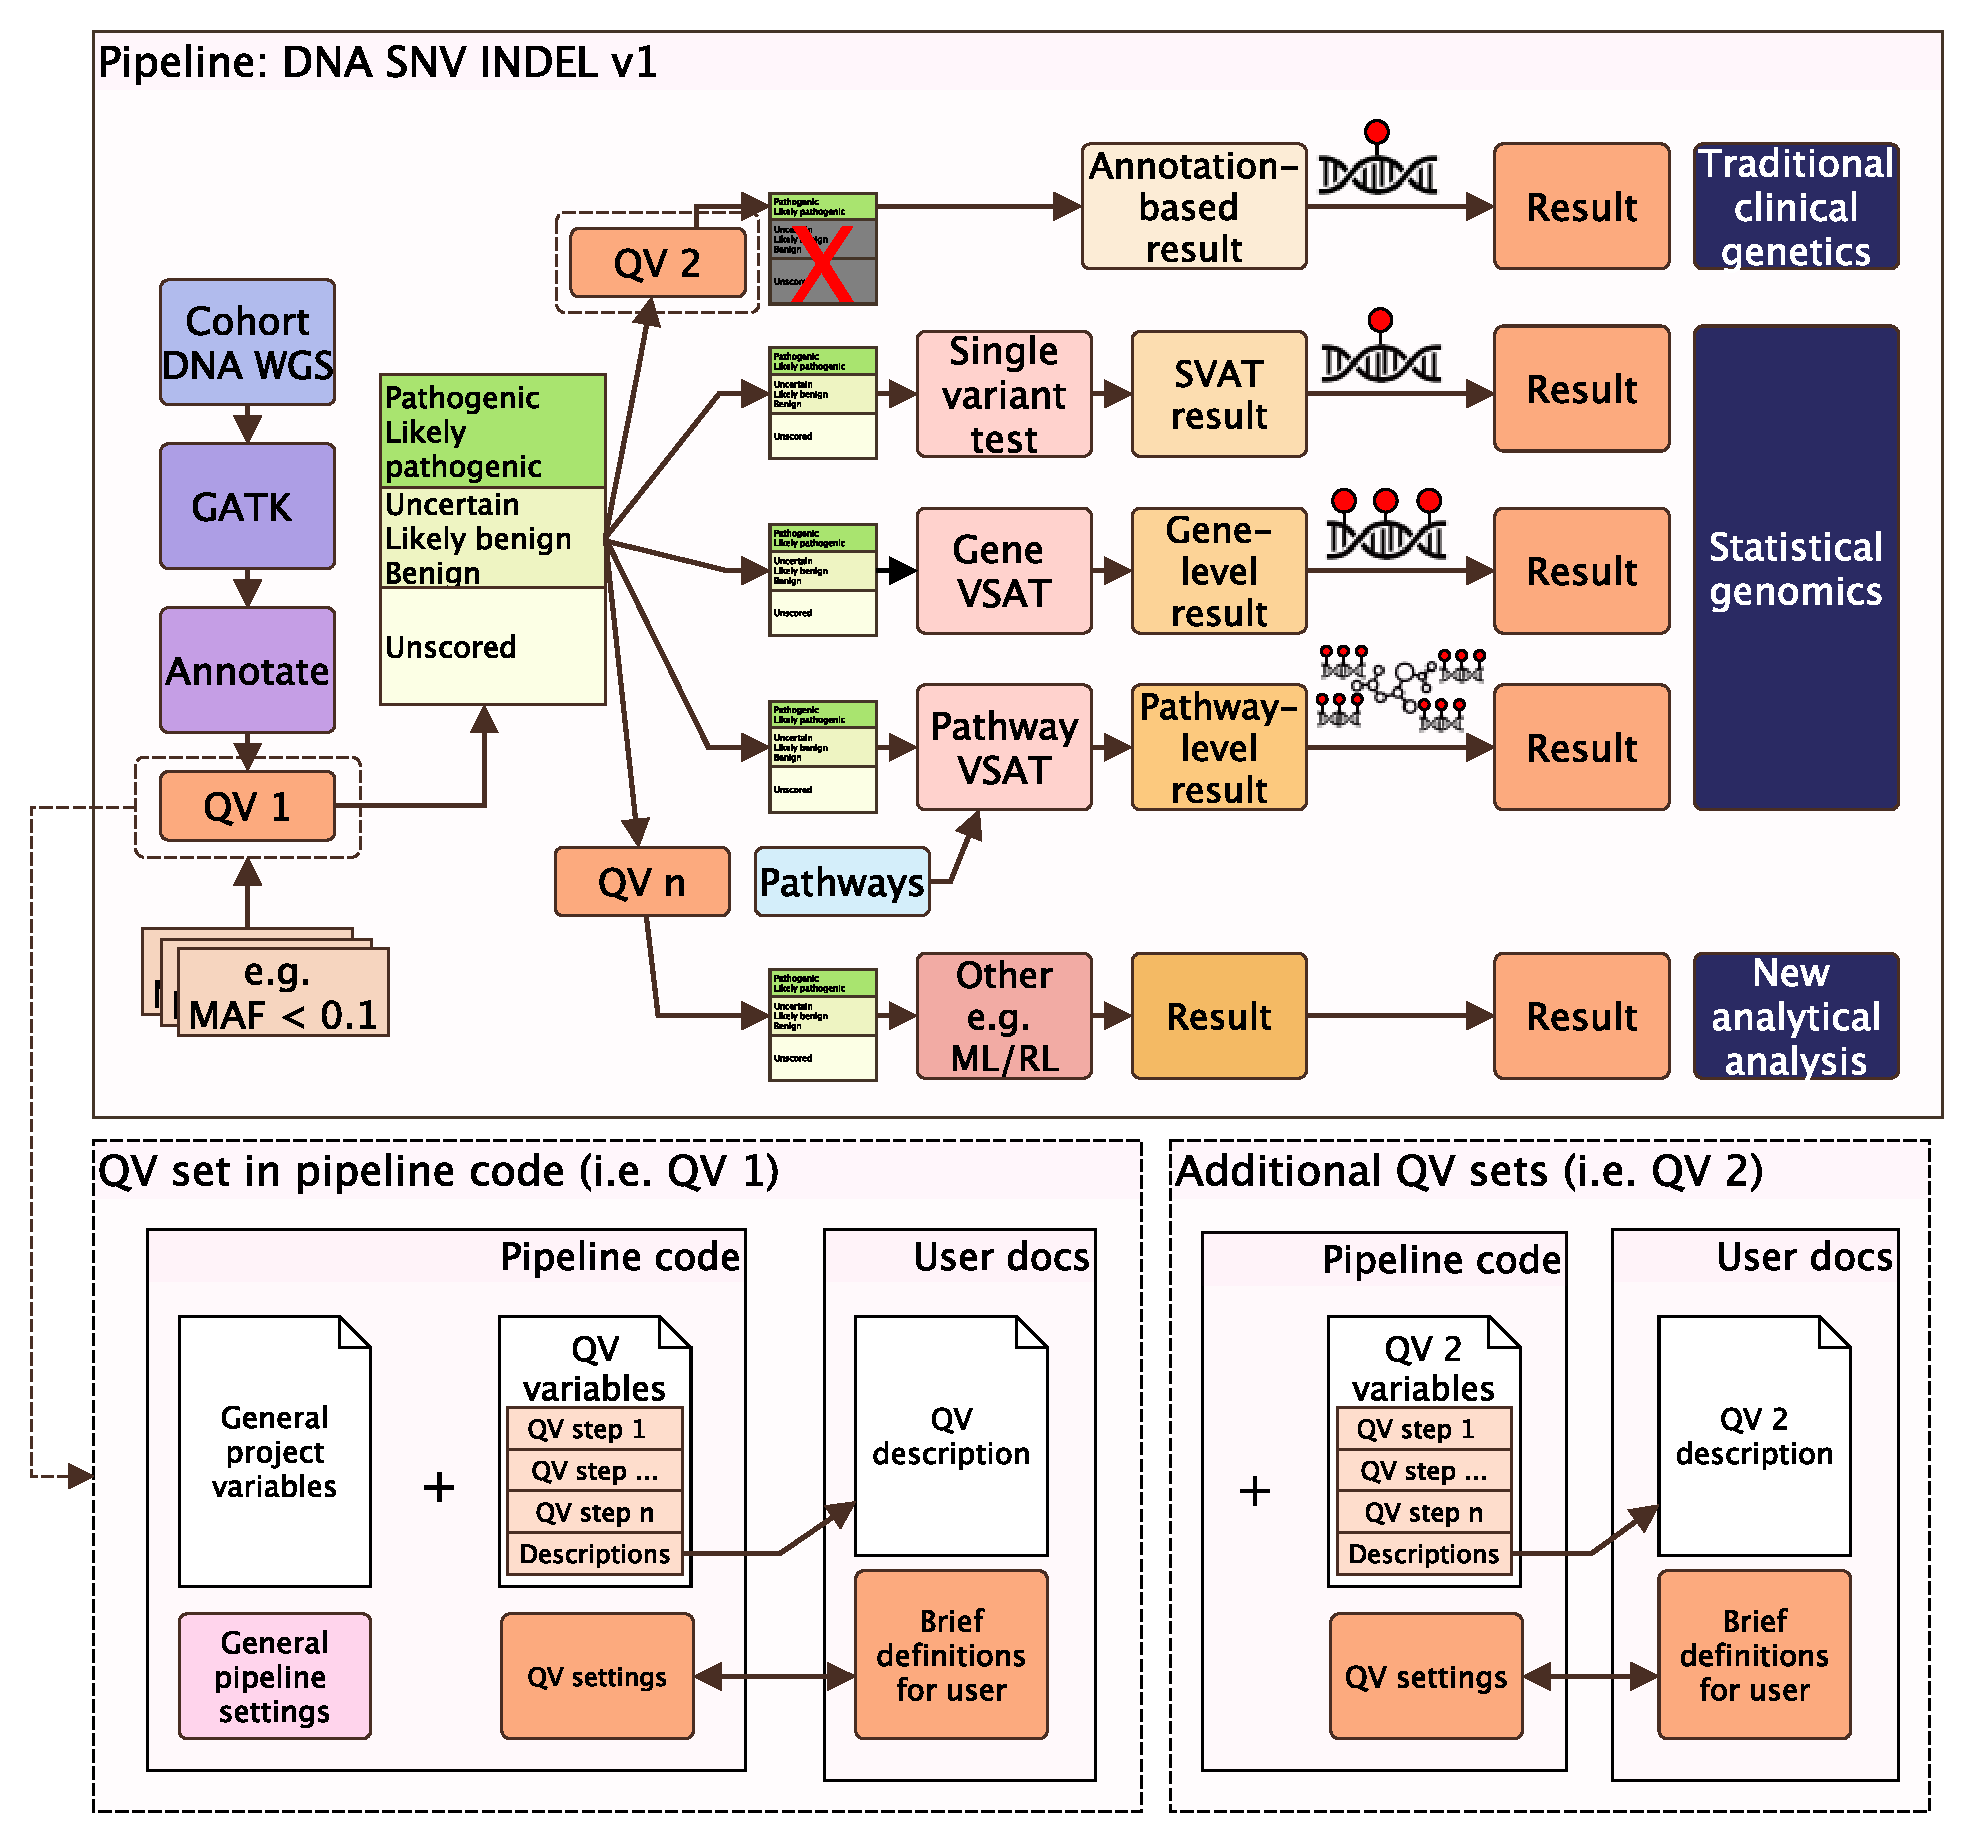
\includegraphics[width=0.85\textwidth]{./images/qv_pipeline_with_file_vcurrent.pdf}
\caption{\DIFaddFL{Summary of the QV application for a WGS pipeline. }\ac{qv}\DIFaddFL{1 and }\ac{qv}\DIFaddFL{2 are applied as sequential protocol steps. In this example, }\ac{qv}\DIFaddFL{2 differs from }\ac{qv}\DIFaddFL{1 by retaining only likely/pathogenic variants (indicated by a red X). The QV file loaded by the analysis pipeline comprises a description field (optional) and a variables field (mandatory). The }\ac{qv} \DIFaddFL{criteria may be distributed across multiple pipeline steps.}}
\label{fig:qv_pipeline_with_file_vcurrent}
\end{figure}
\DIFaddend 

\DIFdelbegin \DIFdel{In a validation study, we demonstrate the use of our }\DIFdelend \DIFaddbegin \subsection{\DIFadd{Usage in a rare disease cohort validation study}}

\DIFadd{We validated the }\DIFaddend \ac{qv} \DIFdelbegin \DIFdel{criteria framework %DIF <  achieve a 100\% match in criterion application when 
compared to the conventional manual approach. 
This analysis was performed }\DIFdelend \DIFaddbegin \DIFadd{framework }\DIFaddend on an in-house rare disease cohort of 940 individuals \DIFdelbegin \DIFdel{, which had been pre-processed for }%DIFDELCMD < \ac{qc}%%%
\DIFdel{. %DIF <  and filtered using a minimal \ac{qv} test set.
We used genome-wide set of variants which was filtering to target rare varaints }\DIFdelend \DIFaddbegin \DIFadd{using }\ac{wes} \DIFadd{comparing a conventional manual implementation with a }\ac{qv}\DIFadd{-based YAML configuration. The analysis targeted rare variants }\DIFaddend (\ac{maf}\DIFdelbegin \DIFdel{$< 0.01$) restricted to }\DIFdelend \DIFaddbegin \DIFadd{~$<0.01$) in }\DIFaddend known disease genes \DIFdelbegin \DIFdel{based on }\DIFdelend \DIFaddbegin \DIFadd{from }\DIFaddend the Genomics England \DIFdelbegin \DIFdel{panel }\DIFdelend ``Primary immunodeficiency or monogenic inflammatory bowel disease\DIFdelbegin \DIFdel{,'' retrieved using our PanelAppRex R repository (}%DIFDELCMD < \url{https://github.com/DylanLawless/PanelAppRex}%%%
\DIFdel{) 
}\DIFdelend \DIFaddbegin \DIFadd{'' panel, retrieved via PanelAppRex }\DIFaddend \cite{lawless_panelapprex_2025}. This \DIFdelbegin \DIFdel{provided us with a prepared dataset of 6026 }\DIFdelend \DIFaddbegin \DIFadd{yielded 6}{\DIFadd{,}}\DIFadd{026 }\DIFaddend candidate variants annotated with 376 information sources\DIFdelbegin \DIFdel{.
The dataset was }\DIFdelend \DIFaddbegin \DIFadd{, }\DIFaddend prepared in R using \DIFdelbegin \DIFdel{GuRu, our }\DIFdelend \DIFaddbegin \DIFadd{the GuRu }\DIFaddend variant interpretation tool \DIFdelbegin \DIFdel{that consolidates all annotation sources and scores variants as candidate causal, and was }\DIFdelend \DIFaddbegin \DIFadd{and }\DIFaddend imported from gVCF \DIFdelbegin \DIFdel{format as output }\DIFdelend \DIFaddbegin \DIFadd{files processed }\DIFaddend by \ac{vep}.

%DIF < Initially, we implemented an \ac{acmg} variant classification protocol \cite{richards2015standards} manually. 
%DIF < We then re-implemented the same protocol using the new framework for \ac{qv} criteria in YAML format. 
\DIFdelbegin \DIFdel{We selected }\DIFdelend \DIFaddbegin \DIFadd{We applied }\DIFaddend the first eight \ac{acmg} criteria for \DIFdelbegin \DIFdel{assigning pathogenicity scores to variants \mbox{%DIFAUXCMD
\cite{richards2015standards}}\hskip0pt%DIFAUXCMD
; six of these were relevant for }\DIFdelend \DIFaddbegin \DIFadd{pathogenicity scoring \mbox{%DIFAUXCMD
\cite{richards2015standards}}\hskip0pt%DIFAUXCMD
, six of which were relevant to }\DIFaddend this cohort. \DIFdelbegin \DIFdel{First, the analysis was performed manually by hard-coding each criterion in the pipeline script, reflecting a typical workflow . Second, the same criteria were imported from the }%DIFDELCMD < \ac{qv} %%%
\DIFdel{YAML filefor the new framework approach, using the file ``qv acmg svnindel criteria 20250225.yaml'' (see }\textbf{\DIFdel{Box \ref{box:acmg_criteria_yaml}}} %DIFAUXCMD
\DIFdel{or }%DIFDELCMD < \url{https://doi.org/10.5281/zenodo.15105594}%%%
\DIFdel{). The outputs from both methods were captured and compared.
}%DIFDELCMD < 

%DIFDELCMD < %%%
\DIFdel{Additional details of the YAML criteria in this }%DIFDELCMD < \ac{qv} %%%
\DIFdel{set included definitions for }\DIFdelend \DIFaddbegin \DIFadd{The manual pipeline encoded each criterion directly, while the }\ac{qv} \DIFadd{workflow read the same definitions from a YAML file. %DIF >  Both produced identical outputs. 
The YAML criteria included }\DIFaddend \texttt{ACMG\_PS1} (\DIFdelbegin \DIFdel{identifying previously established }\DIFdelend \DIFaddbegin \DIFadd{known }\DIFaddend pathogenic amino acid \DIFdelbegin \DIFdel{changes}\DIFdelend \DIFaddbegin \DIFadd{change}\DIFaddend ), \texttt{ACMG\_PS3} (supporting functional \DIFdelbegin \DIFdel{studies with matching inheritance patterns), and }\DIFdelend \DIFaddbegin \DIFadd{evidence), }\DIFaddend \texttt{ACMG\_PS5} (\DIFdelbegin \DIFdel{covering compound heterozygositywith high-impact variants). The criteria for }\texttt{\DIFdel{ACMG\_PM2}} %DIFAUXCMD
\DIFdel{and }\texttt{\DIFdel{ACMG\_PM3}} %DIFAUXCMD
\DIFdel{assess variant frequency and in trans occurrences, respectively, while }\DIFdelend \DIFaddbegin \DIFadd{compound heterozygosity), and frequency- and segregation-based criteria (}\texttt{\DIFadd{PM2}}\DIFadd{, }\texttt{\DIFadd{PM3}}\DIFadd{). Criteria }\DIFaddend \texttt{PS2} and \texttt{PS4} were not applicable \DIFdelbegin \DIFdel{to }\DIFdelend \DIFaddbegin \DIFadd{in }\DIFaddend this cohort.

%DIF <  Individual steps within the \ac{qv} criteria can be further classified for organisational purposes using simple labels such as ``QC'' and ``filter''. For example, filtering thresholds (e.g. allele frequency > 0.1 in a cohort, < 0.1 in gnomAD) may be applied directly to exclude variants, while annotation-based criteria (e.g. QC flags) might not remove variants outright but instead inform downstream analyses that integrate multiple \ac{qv} filters.
\DIFaddbegin \subsection{\DIFadd{Usage in a GWAS validation study}}
\DIFadd{We next applied the }\ac{qv} \DIFadd{criteria framework to a }\ac{gwas} \DIFadd{using HapMap3 Phase 3 (R3) consensus genotypes on 1397 individuals \mbox{%DIFAUXCMD
\cite{2020fairleyInternationalGenomeSample}}\hskip0pt%DIFAUXCMD
. Again, two pipelines were executed with identical inputs and parameters: one hard-coded and one driven by the }\ac{qv}  \DIFadd{file.
This }\ac{qv}  \DIFadd{set defined common GWAS thresholds: restriction to autosomal, biallelic SNPs; minimum sample call rate of $95\%$; variant call rate of $95\%$; minor allele frequency $\geq 1\%$; and Hardy–Weinberg equilibrium $p \geq 1\times10^{-6}$. After quality control, variants were LD-pruned and principal components (PC1–PC10) were computed, with sex included as an additional covariate. Logistic regression under an additive model was then performed with a binary simulated phenotype using PLINK.
The outputs of the two pipelines were captured and compared across each main PLINK stage. Manhattan plots, }\ac{pca} \DIFadd{plots, and }\texttt{\DIFadd{md5}} \DIFadd{checksums were used to confirm exact reproducibility between the hard-coded and QV-driven analyses.
}\DIFaddend 

\DIFdelbegin %DIFDELCMD < \begin{tcolorbox}[
%DIFDELCMD <     colback=white!0,
%DIFDELCMD <     colframe=black,
%DIFDELCMD <     boxrule=1pt,
%DIFDELCMD <     arc=1mm,
%DIFDELCMD <     outer arc=1mm,
%DIFDELCMD <     title=\textbf{\refstepcounter{myboxcounter}\label{box:acmg_criteria_yaml}Box \themyboxcounter: qv\_files/acmg\_criteria.yaml}
%DIFDELCMD < ]
%DIFDELCMD < \begin{verbatim}
%DIFDELCMD < %%%
%DIFAUXCMD NEXT
\DIFmodbegin
\begin{DIFverbatim}[alsolanguage=DIFcode]
%DIF < qv_set_id: acmg_sf_v3.2
%DIF < -
%DIF < acmg_pvs1:
%DIF <   description_technical: >
%DIF <     Null variants (IMPACT = HIGH) in genes where 
%DIF <     loss-of-function causes disease.
%DIF <     Includes homozygous variants, dominant inheritance, 
%DIF <     and compound heterozygous cases.
%DIF <     Compound heterozygosity is considered when both 
%DIF <     variants are HIGH impact. WARNING: Not phase checked.
%DIF <   logic: "or"
%DIF <   conditions:
%DIF <     - condition:
%DIF <         field: IMPACT
%DIF <         value: "HIGH"
%DIF <         operator: "=="
%DIF < ...
%DIF < shasum -a 256 acmg_criteria.yaml | fold -w 32
%DIF < d91fde41a5fff48631adecba38773d61
%DIF < 9ae8cd5cff9b9b42ef7f5efbd6bbfcdf
%DIF < acmg_criteria.yaml
\end{DIFverbatim}
\DIFmodend %DIFAUXCMD
%DIFDELCMD < \end{verbatim}
%DIFDELCMD < \end{tcolorbox}
%DIFDELCMD < %%%
\DIFdelend \DIFaddbegin \DIFadd{For benchmarking, }\ac{md5} \DIFadd{checksums were uniquely reported for the GWAS study because PLINK output files are exactly reproducible between runs. In contrast, VCF files used in the other validation studies include variable header fields such as BCFtools view command with a timestamp, which changes with each run and alters the }\ac{md5} \DIFadd{value. For those cases, we instead report variant count and content.
}\DIFaddend 

\DIFdelbegin \section{\DIFdel{Results}}
%DIFAUXCMD
\addtocounter{section}{-1}%DIFAUXCMD
\DIFdelend \subsection{\DIFdelbegin \DIFdel{Validation Case Study}\DIFdelend \DIFaddbegin \DIFadd{Usage in a WGS validation study with GIAB and Exomiser}\DIFaddend }
\DIFaddbegin \DIFadd{We next applied the }\ac{qv} \DIFadd{framework to a }\ac{wgs} \DIFadd{trio analysis using the Genome In A Bottle Chinese Trio (HG005-HG007, PRJNA200694, GRCh38 v4.2.1) of the National Institute of Standards and Technology \mbox{%DIFAUXCMD
\cite{2022wagnerBenchmarkingChallengingSmall}}\hskip0pt%DIFAUXCMD
. 
Two pipeline phases were executed with identical inputs and parameters: one hard-coded and one driven by the }\ac{qv} \DIFadd{file.
Both phases applied identical }\ac{qc} \DIFadd{and study filters and included a gene-panel style analysis using the paediatric disorders panel (panel 486; 3}{\DIFadd{,}}\DIFadd{853 genes \mbox{%DIFAUXCMD
\cite{lawless_panelapprex_2025}}\hskip0pt%DIFAUXCMD
). 
The upstream processing used BCFtools for region restriction using BED overlap, site-level thresholds on QUAL and INFO/DP (using computed site depth from per-sample FORMAT/DP when absent), and per-sample thresholds on FORMAT/DP and FORMAT/GQ with exclusion of missing genotypes. 
Composite criteria were applied to require either all samples to pass or at least one sample to pass. 
The downstream filtered trio }\ac{vcf} \DIFadd{was analysed with Exomiser using the same trio }\texttt{\DIFadd{.ped}} \DIFadd{input and without using }\ac{hpo} \DIFadd{terms.
}\DIFaddend 

\DIFdelbegin \DIFdel{We validated our }\DIFdelend \DIFaddbegin \section{\DIFadd{Results}}
\subsection{\DIFadd{Validation rare disease cohort case study}}
\DIFadd{We validated the }\DIFaddend \ac{qv} \DIFdelbegin \DIFdel{protocol using }\DIFdelend \DIFaddbegin \DIFadd{framework using }\ac{wes} \DIFadd{analysis with }\DIFaddend \ac{acmg}-based criteria \DIFdelbegin \DIFdel{for }\DIFdelend \DIFaddbegin \DIFadd{on }\DIFaddend a rare disease cohort of 940 individuals\DIFdelbegin \DIFdel{. 
We then conducted the variant classification using two approaches: a conventional manual method with hard-coded criteria, and our new }\DIFdelend \DIFaddbegin \DIFadd{, comparing a conventional pipeline with parameters defined internally (QV manual) to the new external }\DIFaddend YAML-based implementation \DIFaddbegin \DIFadd{(QV yaml).
}\DIFaddend As shown in \textbf{Figure \DIFdelbegin \DIFdel{\ref{fig:qv_pipeline_with_file_vcurrent_guru_case_study_result} (B)}\DIFdelend \DIFaddbegin \DIFadd{\ref{fig:guru_singlecase_validation_of_yaml_vs_manual}}\DIFaddend }, 
the outputs from both methods were identical, demonstrating a 100\% match. This confirmed that our framework of a standalone, shareable, \ac{qv} criteria file can be imported and applied programmatically with equivalent accuracy, providing a reproducible resource that is adaptable across different pipelines and programming environments.

%DIF <  Results/Methods: Figure showing pipeline and validation case study.
\DIFdelbegin %DIFDELCMD < \begin{figure}[!h]
%DIFDELCMD < \centering
%DIFDELCMD < \begin{minipage}{0.85\textwidth}
%DIFDELCMD < \raggedright %%%
\DIFdelFL{A}%DIFDELCMD < \\[0.5ex]
%DIFDELCMD < 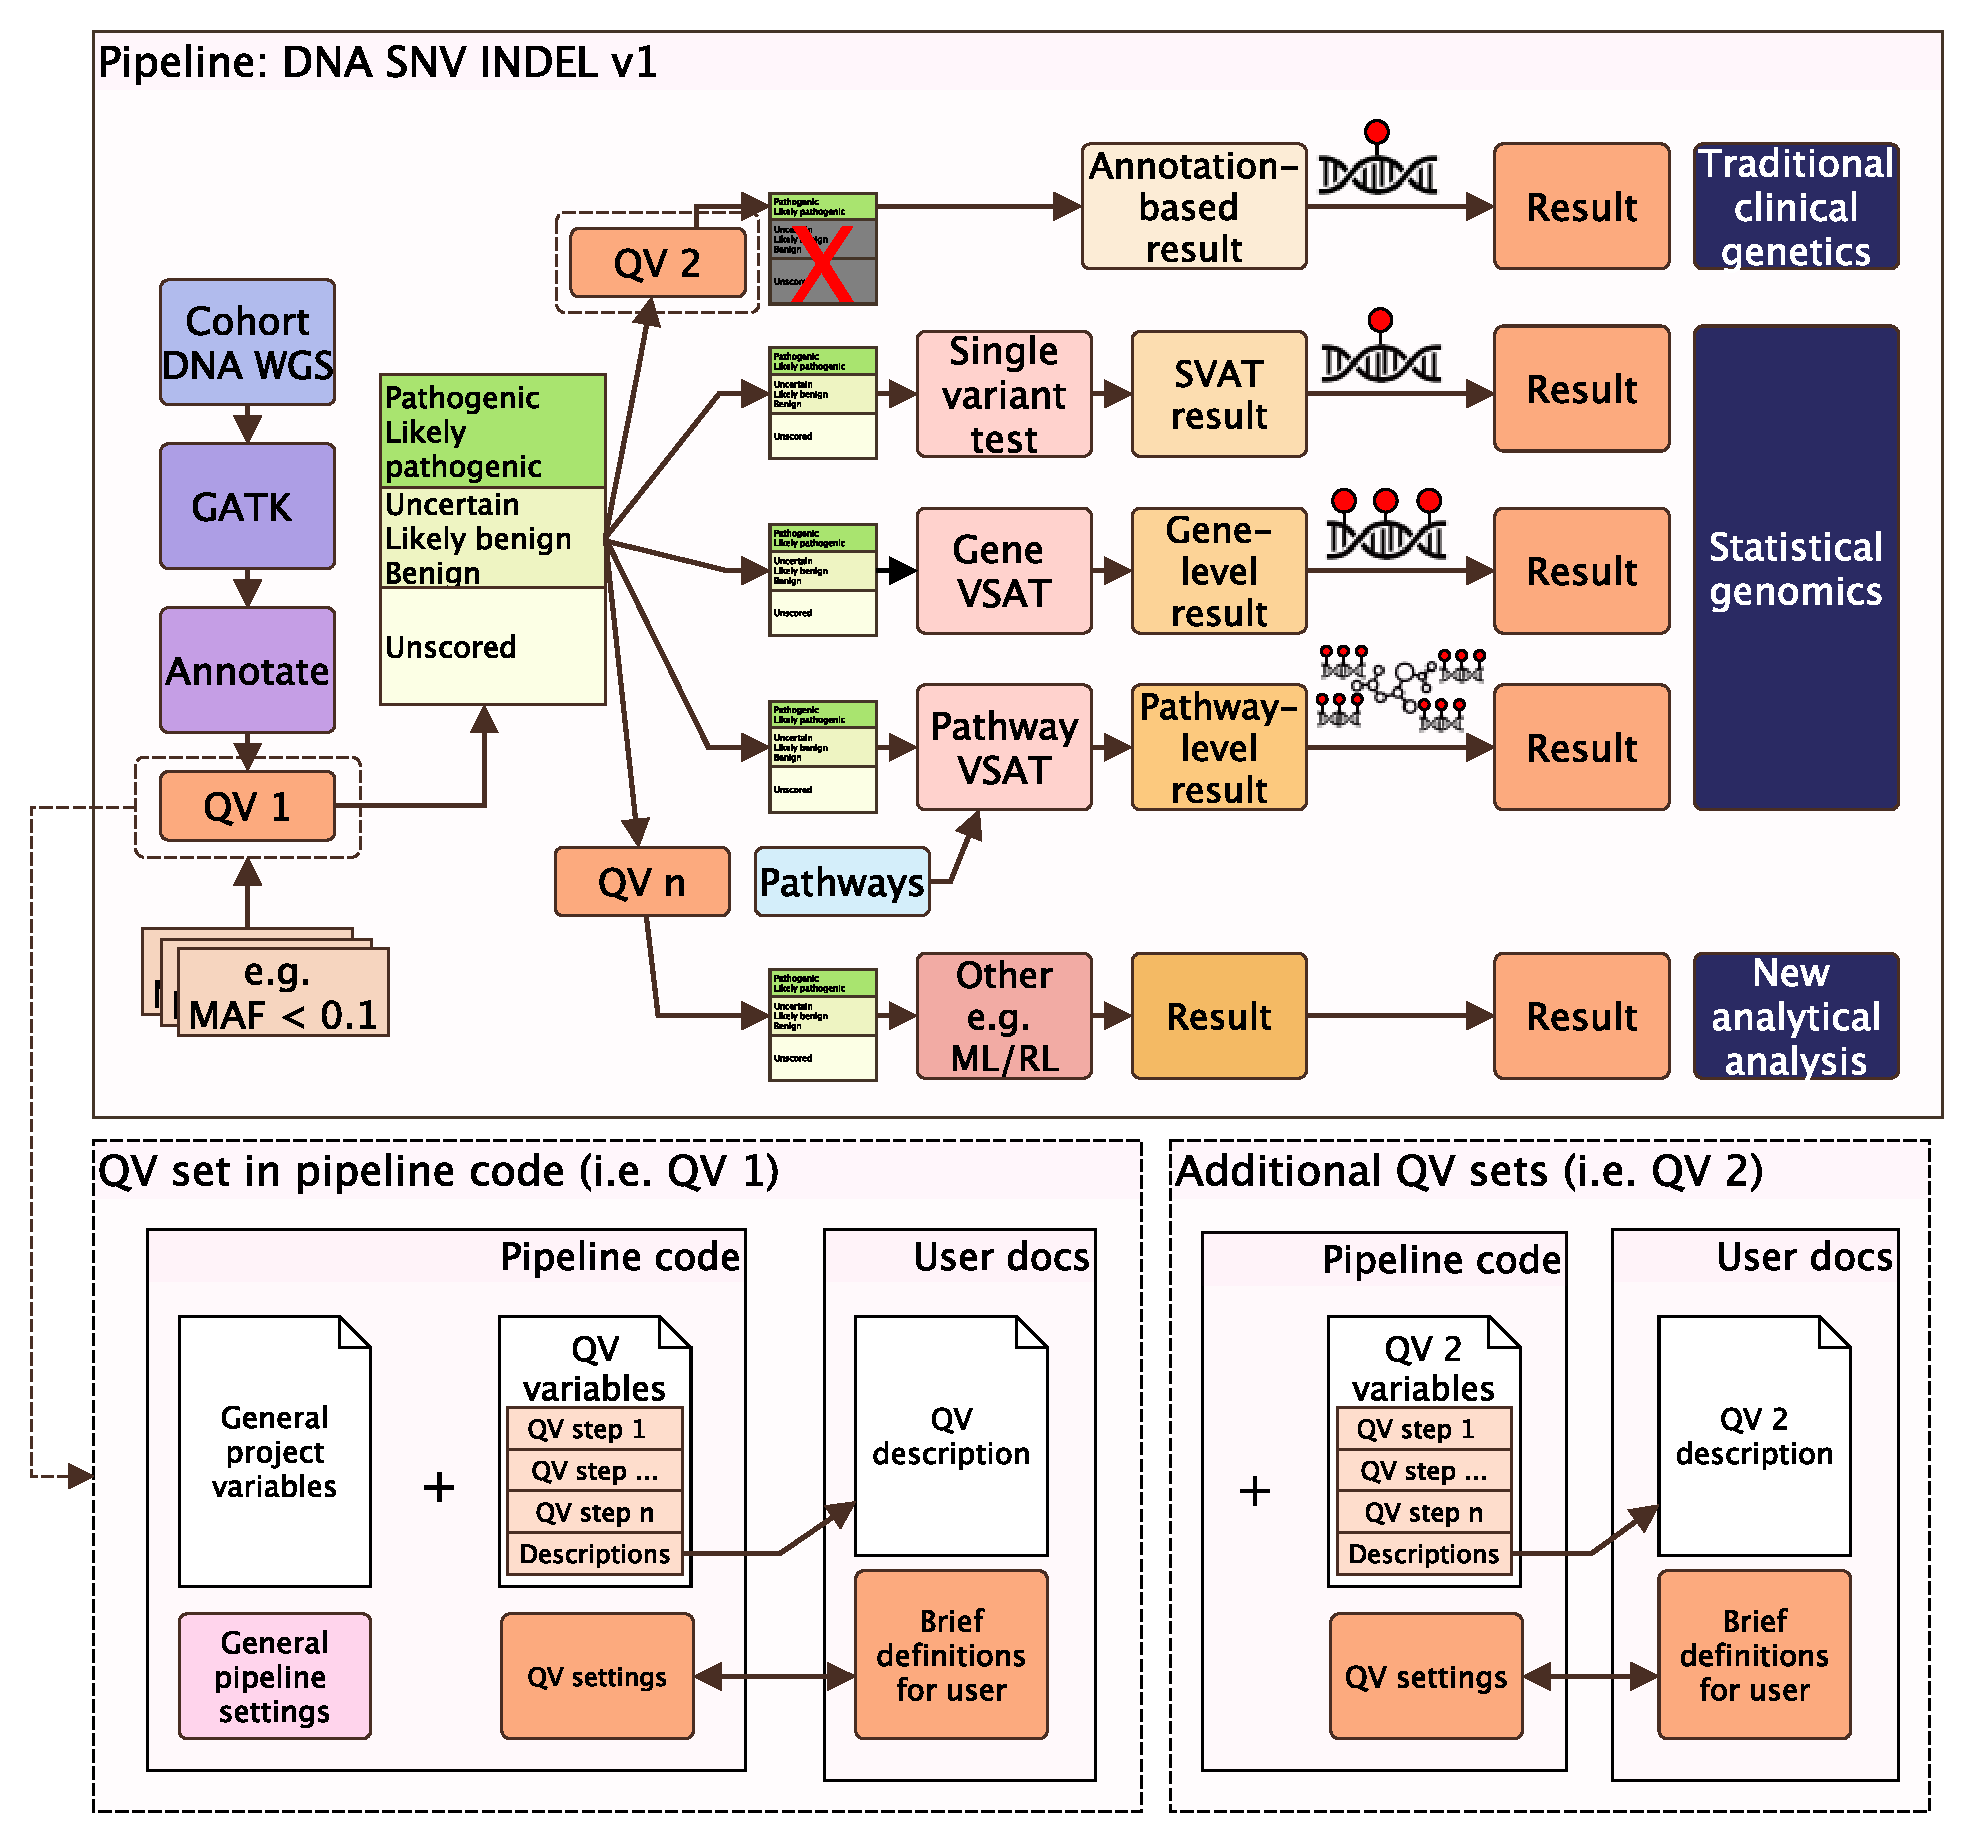
\includegraphics[width=\textwidth]{./images/qv_pipeline_with_file_vcurrent.pdf}
%DIFDELCMD < \end{minipage}\\[-2ex]
%DIFDELCMD < \begin{minipage}{0.9\textwidth}
%DIFDELCMD < \raggedright %%%
\DIFdelFL{B}%DIFDELCMD < \\[0.5ex]
%DIFDELCMD < 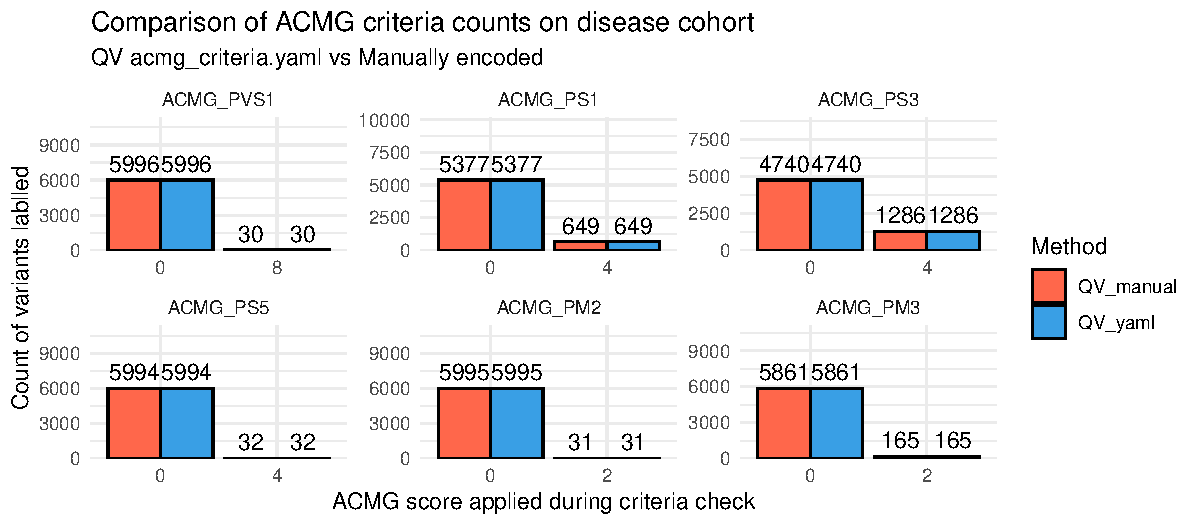
\includegraphics[width=\textwidth]{./images/Guru_singlecase_validation_of_yaml_vs_manual.pdf}
%DIFDELCMD < \end{minipage}
%DIFDELCMD <     %%%
%DIFDELCMD < \caption{%
{%DIFAUXCMD
\DIFdelFL{Summary of the QV application for a WGS pipeline. In panel (A), }%DIFDELCMD < \ac{qv}%%%
\DIFdelFL{1 and }%DIFDELCMD < \ac{qv}%%%
\DIFdelFL{2 are presented as sequentially piped protocol steps. In this example, }%DIFDELCMD < \ac{qv}%%%
\DIFdelFL{2 differs from }%DIFDELCMD < \ac{qv}%%%
\DIFdelFL{1 by retaining only likely/pathogenic variants (indicated by a red X). The QV file loaded by the analysis pipeline comprise a description field (optional) and a variables field (mandatory). The }%DIFDELCMD < \ac{qv} %%%
\DIFdelFL{criteria may be spread throughout the pipeline.
    (B) Validation case study using an }%DIFDELCMD < \ac{acmg} %%%
\DIFdelFL{criteria subset, demonstrating a 100\% match between manually encoded and standalone YAML-based }%DIFDELCMD < \ac{qv} %%%
\DIFdelFL{(}\texttt{\DIFdelFL{qv\_files/acmg\_criteria.yaml}}%DIFAUXCMD
\DIFdelFL{) for assigning pathogenicity scores.}}
    %DIFAUXCMD
%DIFDELCMD < \label{fig:qv_pipeline_with_file_vcurrent_guru_case_study_result}
%DIFDELCMD < \end{figure}
%DIFDELCMD < %%%
\DIFdelend \DIFaddbegin \subsection{\DIFadd{Validation in a common variant GWAS}}
\DIFadd{To demonstrate the integration of the }\ac{qv} \DIFadd{framework with established best practices in }\ac{gwas} \DIFadd{\mbox{%DIFAUXCMD
\cite{2021uffelmannGenomewideAssociationStudies}}\hskip0pt%DIFAUXCMD
, we validated it in a standard HapMap3 Phase 3 }\ac{gwas} \DIFadd{by again running two equivalent analyses: a conventional pipeline with parameters defined internally and a YAML-based implementation that externalised all settings.
As shown in }\textbf{\DIFadd{Figure~\ref{fig:hapmap_gwas_validation}}}\DIFadd{, the Manhattan and }\ac{pca} \DIFadd{plots were identical between the two methods, and the }\ac{md5} \DIFadd{checksums of all PLINK outputs matched exactly. These results confirm that }\ac{qv} \DIFadd{parameterisation reproduces the original workflow precisely while improving clarity, transparency, and reusability.
}\DIFaddend 

\subsection{\DIFdelbegin \DIFdel{Implications}%DIFDELCMD < \MBLOCKRIGHTBRACE
%DIFDELCMD < %%%
%DIF <  Framework: Highlight the clinical relevance and benefits.
\DIFdel{In the validation }\DIFdelend \DIFaddbegin \DIFadd{Validation in a WGS }\DIFaddend study \DIFdelbegin \DIFdel{, we applied }%DIFDELCMD < \ac{acmg} %%%
\DIFdel{criteria for variant interpretation}\DIFdelend \DIFaddbegin \DIFadd{with GIAB and Exomiser}}
\DIFadd{To demonstrate the ease and benefit of using }\ac{qv} \DIFadd{parameterisation in established }\ac{wgs} \DIFadd{analysis pipelines, we conducted a trio validation study using the }\ac{giab} \DIFadd{Chinese Trio (HG005-HG007, GRCh38 v4.2.1) and the Exomiser tool for variant annotation and interpretation \mbox{%DIFAUXCMD
\cite{2020ciprianiImprovedPhenotypeDrivenTool}}\hskip0pt%DIFAUXCMD
. 
Two equivalent analyses were run: one with hard-coded thresholds and one using an external }\ac{qv} \DIFadd{YAML file specifying the same parameters. Both applied identical }\ac{qc} \DIFadd{and study filters and restricted analysis to the PanelAppRex paediatric disorders panel (3}{\DIFadd{,}}\DIFadd{853~genes). Results were identical: variant counts matched at each step, and Exomiser outputs produced the same candidate genes and variants}\DIFaddend . \DIFdelbegin \DIFdel{In clinical genetics,for instance, the resulting output can be used to retrieve candidate pathogenic variantsusing }%DIFDELCMD < \ac{acmg} %%%
\DIFdel{scoring methods \mbox{%DIFAUXCMD
\cite{richards2015standards, tavtigian2020fitting}}\hskip0pt%DIFAUXCMD
. Application of additional }\DIFdelend \DIFaddbegin \textbf{\DIFadd{Figure~\ref{fig:qv_exomiser_validation}}} \DIFadd{shows this agreement.
This validation confirms that a shareable }\DIFaddend \ac{qv} \DIFdelbegin \DIFdel{sets, such as the widely used }%DIFDELCMD < \ac{acmg} \ac{sf} %%%
\DIFdel{set for clinical reporting \mbox{%DIFAUXCMD
\cite{miller2023acmg}}\hskip0pt%DIFAUXCMD
, can be used to confirm any secondary findings}\DIFdelend \DIFaddbegin \DIFadd{file reproduces the full variant interpretation workflow exactly, while aligning with established variant effect predictors and interpretation tools \mbox{%DIFAUXCMD
\cite{2024riccioVariantEffectPredictors, 2020ciprianiImprovedPhenotypeDrivenTool, 2020holtgreweVarFishComprehensiveDNA}}\hskip0pt%DIFAUXCMD
.
Benchmarking showed that QV files introduce no computational overhead and scale equivalently to conventional implementations 
(}\textbf{\DIFadd{Supplemental \ref{sec:benchmark}}}\DIFadd{, 
}\textbf{\DIFadd{Figure \ref{fig:benchmark_preprocess_time_bars_by_step_elapsed}}}\DIFadd{)}\DIFaddend .

\DIFdelbegin \DIFdel{In a clinical setting it is necessary to bridge the gap between technical detail and lay understanding. By explicitly documenting variant qualifying criteria and making }\DIFdelend \DIFaddbegin \subsection{\DIFadd{Implications}}
\subsubsection*{\DIFadd{General applicability and reproducibility}}
\DIFadd{Across validation studies, the }\DIFaddend \ac{qv} \DIFdelbegin \DIFdel{data accessible, our framework builds trust and supports meaningful }%DIFDELCMD < \ac{ppi} %%%
\DIFdel{\mbox{%DIFAUXCMD
\cite{morris_answer_2011}}\hskip0pt%DIFAUXCMD
. The }\DIFdelend \DIFaddbegin \DIFadd{framework reproduced conventional workflows in which parameters are embedded within scripts, while externalising those same variables into a portable, shareable format. The framework itself performs no filtering, calling, annotation, or interpretation, but provides a machine-readable layer for defining and reusing the qualifying variables that underpin these analyses. It complements tools such as GATK and BCFtools for processing, Ensembl VEP, SnpEff, FAVOR, and WGSA for variant effect prediction \mbox{%DIFAUXCMD
\cite{2024riccioVariantEffectPredictors}}\hskip0pt%DIFAUXCMD
, and Exomiser and VarFish for interpretation \mbox{%DIFAUXCMD
\cite{2020ciprianiImprovedPhenotypeDrivenTool, 2020holtgreweVarFishComprehensiveDNA}}\hskip0pt%DIFAUXCMD
, by making their analytic criteria explicit.
}

\subsubsection*{\DIFadd{Scalability and interoperability with genomic tools}}
\DIFadd{The validation studies, covering clinical interpretation, genome-wide association analysis, and WGS trio interpretation, demonstrate that the }\DIFaddend \ac{qv} \DIFdelbegin \DIFdel{file adapts by integrating the main criteria variables with optionally dedicated fields for both technical description and }%DIFDELCMD < \ac{ppi} %%%
\DIFdel{description. This approach captures the analysis intent defined by the }\DIFdelend \DIFaddbegin \DIFadd{framework generalises across distinct genomic contexts without altering analytical outcomes or adding computational overhead. The format further allows users to define, combine, and extend their own }\DIFaddend \ac{qv} \DIFdelbegin \DIFdel{set creator and embeds patient preferences from the start. }\DIFdelend \DIFaddbegin \DIFadd{sets using simple declarative syntax, providing a scalable approach for reproducible genomics.
}\DIFaddend 

\DIFaddbegin \subsubsection*{\DIFadd{Traceability and confirmation of applied clinical standards}}
\DIFadd{Each }\ac{qv} \DIFadd{file includes a persistent identifier and checksum that can be stored in }\ac{ehr} \DIFadd{or laboratory systems such as EPIC, Cerner, Clinisys, or REDCap. This links each patient’s analysis (including any associated }\ac{ppie} \DIFadd{input) to the exact }\ac{qv} \DIFadd{set used, enabling transparent, auditable, and }\ac{fair}\DIFadd{-compliant reporting.  
A clinician or molecular pathologist viewing a result in EPIC or Cerner can access the linked }\texttt{\DIFadd{qv\_set\_id}} \DIFadd{to verify the applied standards and filtering criteria. Automated genomic reports should include these details by default, ensuring full traceability without requiring access to the pipeline.  
}\DIFaddend For example, \DIFdelbegin \DIFdel{patient preferences recorded in }\DIFdelend \DIFaddbegin \DIFadd{if a patient asks whether their genome was screened for breast cancer due to variants in }\textit{\DIFadd{BRCA1}} \DIFadd{or }\textit{\DIFadd{BRCA2}}\DIFadd{, }\DIFaddend the \DIFdelbegin %DIFDELCMD < \ac{ppi} %%%
\DIFdel{description can be automatically incorporated into a genetic report without additional interpretation, ensuring clarity and consistency throughout the analysis. This transparency guarantees that both experts and laypersons receive information in a format suited to their needs, thereby improving diagnostic traceability and accelerating the translation of genetic research into clinical practice}\DIFdelend \DIFaddbegin \ac{ehr}\DIFadd{-linked report referencing ``qv acmg sf v3.3 20250828.json'' confirms that the }\ac{acmg} \DIFadd{secondary findings guideline (v3.3) \mbox{%DIFAUXCMD
\cite{miller2023acmg} }\hskip0pt%DIFAUXCMD
was applied, including its defined gene set, thresholds, version, and standard}\DIFaddend .  

\DIFdelbegin %DIFDELCMD < \FloatBarrier
%DIFDELCMD < 

%DIFDELCMD < %%%
\DIFdelend \section{Summary}
This paper introduces a framework for integrating qualifying variants into genomic analysis pipelines, enhancing reproducibility, interpretability and the seamless translation of research findings into clinical practice.

\DIFaddbegin \FloatBarrier

\DIFaddend \section{Funding}
This project was supported through the grant Swiss National Science Foundation  320030\_201060, and NDS-2021-911 (SwissPedHealth) from the Swiss Personalized Health Network and the Strategic Focal Area `Personalized Health and Related Technologies' of the ETH Domain (Swiss Federal Institutes of Technology).

\section{Acknowledgements}
Acknowledgements We would like to thank all the patients and families who have been providing advice on SwissPedHealth and its projects, as well as the clinical and research teams at the participating institutions.

\section{Contributions}
DL designed the work and contributed to the manuscript.
AS, SB, VS, DH, SÖ, JA\DIFaddbegin \DIFadd{, SF }\DIFaddend contributed to the manuscript.
\DIFdelbegin \DIFdel{JF, SF, LJS }\DIFdelend \DIFaddbegin \DIFadd{LJS and JF }\DIFaddend supervised the work, manuscript, and applied for funding.

\section{Competing interests}
The authors declare no competing interests.

\section{Ethics statement}
\DIFdelbegin \DIFdel{Summary statistics were used from studies which have been previously reported and }\DIFdelend \DIFaddbegin \DIFadd{The projects were }\DIFaddend approved by the respective ethics committees of all participating centers (Cantonal Ethics Committee Bern, approval number KEK-029/11) and the study was conducted in accordance with the Declaration of Helsinki.

\bibliographystyle{unsrtnat}
\bibliography{references} 
\DIFaddbegin \clearpage
\FloatBarrier

%DIF > \\\\\\\\\\\\\\\\\\\\\\\\\\\\
\beginsupplement
\section{\DIFadd{Supplemental}} \label{Supplemental_text}
\textbf{\DIFadd{Application of qualifying variants for genomic analysis.}}

\subsection{\DIFadd{Validation study figures}}

\begin{figure}[h]
\centering
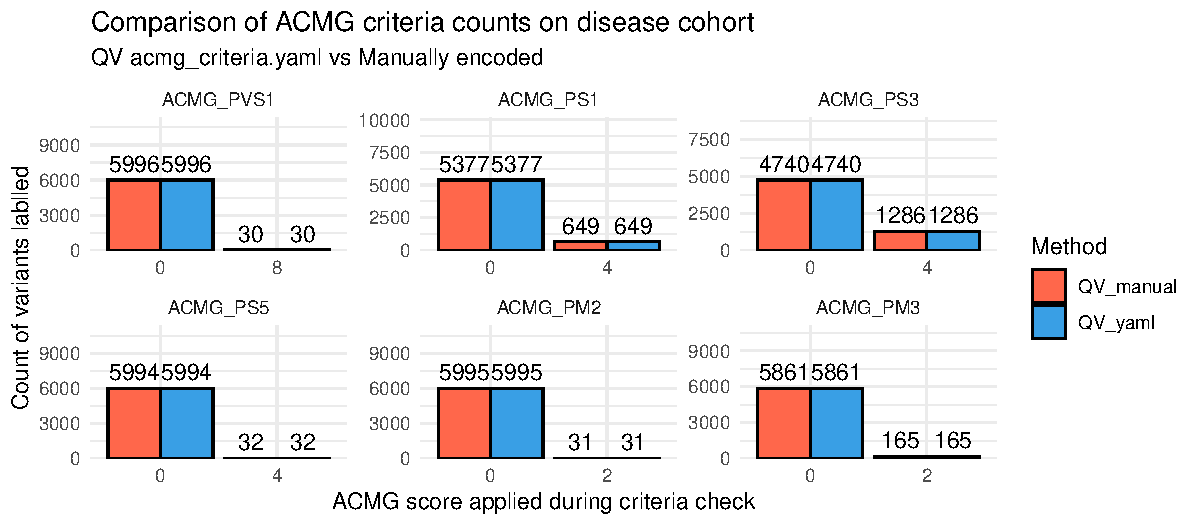
\includegraphics[width=0.9\textwidth]{./images/Guru_singlecase_validation_of_yaml_vs_manual.pdf}
\caption{\DIFaddFL{Validation case study of a rare disease cohort of 940 WES individuals using an }\ac{acmg} \DIFaddFL{criteria subset, demonstrating a 100\% match between manually encoded and standalone YAML-based }\ac{qv} \DIFaddFL{for assigning pathogenicity scores.}}
\label{fig:guru_singlecase_validation_of_yaml_vs_manual}
\end{figure}


\begin{figure}[h]
\centering
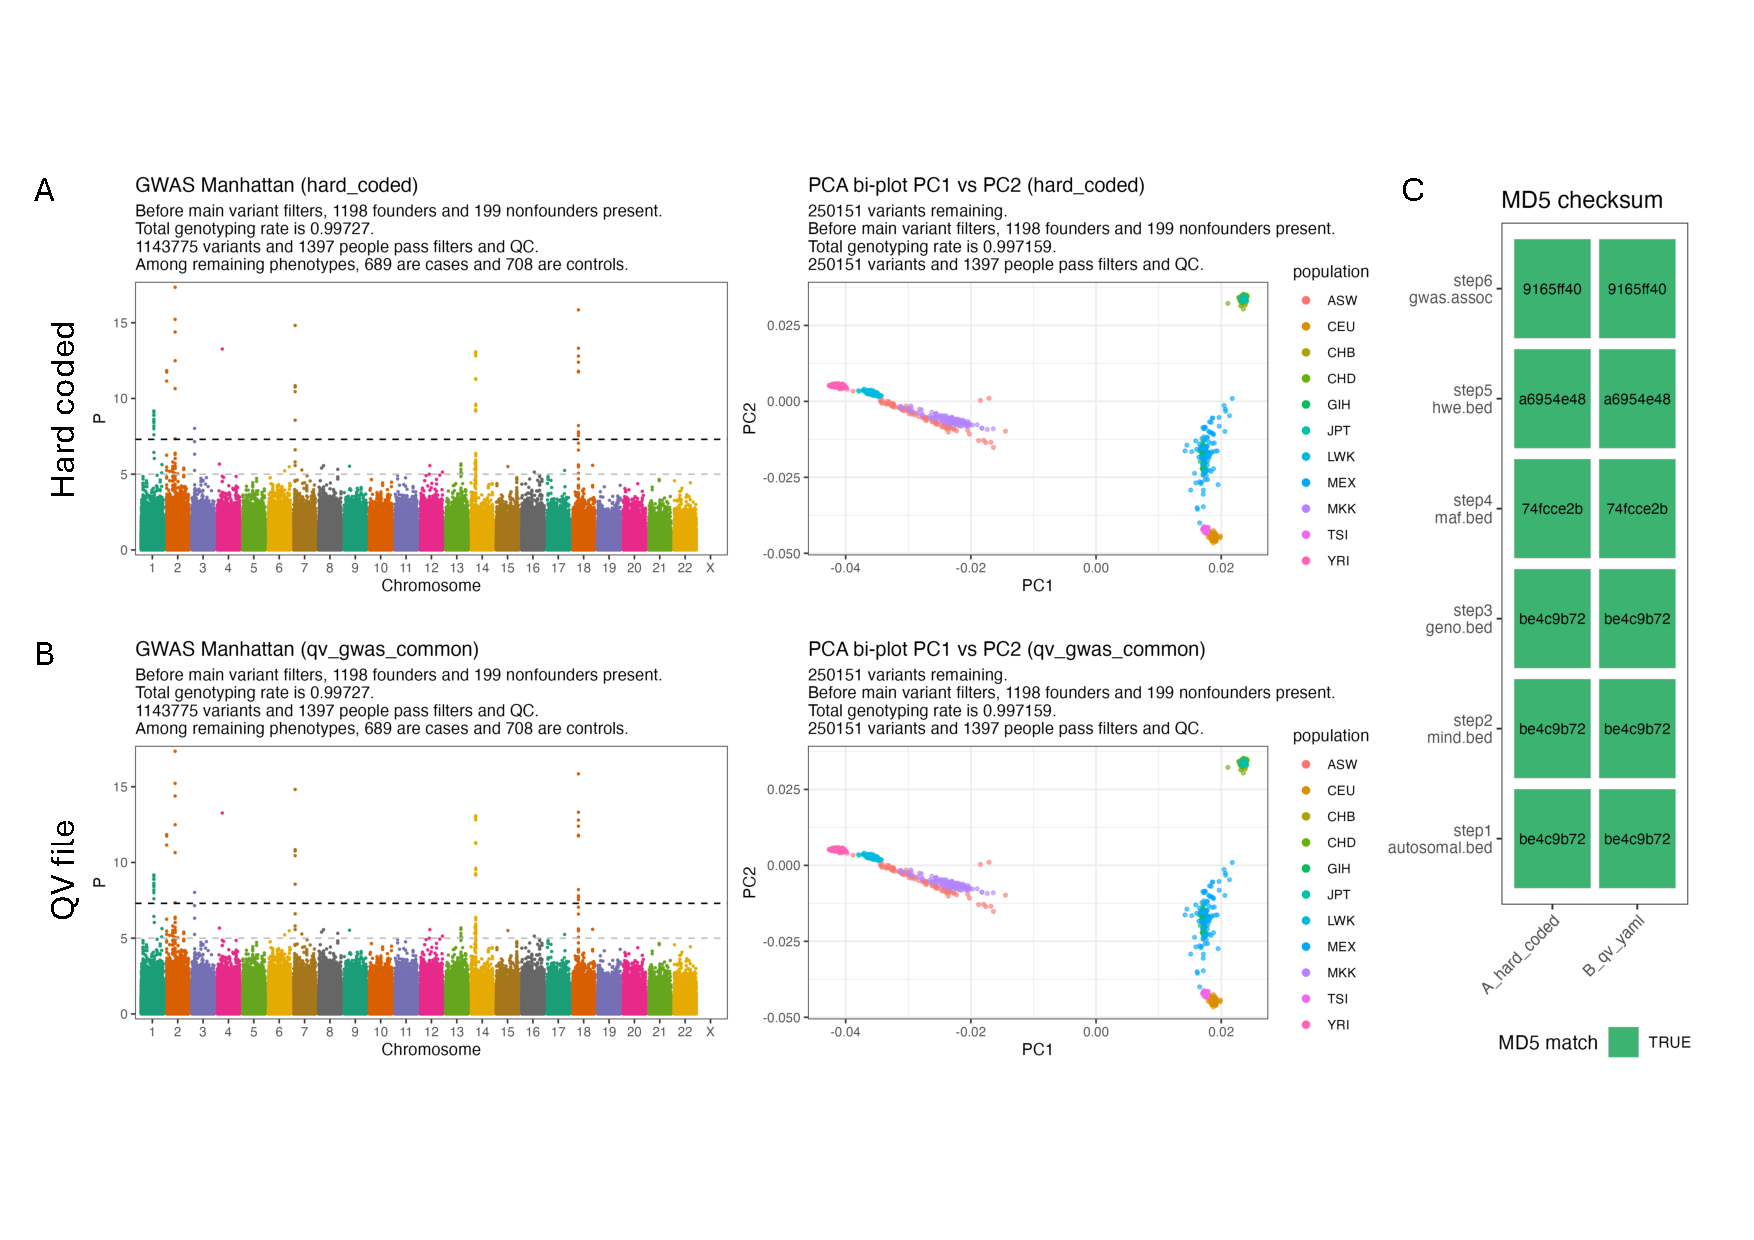
\includegraphics[width=\textwidth]{./images/hapmap_gwas_validation.pdf}
\caption{\DIFaddFL{Validation in GWAS using QV parameterisation. 
(A) }\ac{gwas} \DIFaddFL{of simulated binary phenotypes in HapMap3 Phase 3 (R3) using a traditional variable embedded pipeline. Shown are the Manhattan plot of logistic regression results (left) and correction for population structure with principal component analysis (PC1 vs PC2, right). 
(B) Identical }\ac{gwas} \DIFaddFL{using a }\ac{qv} \DIFaddFL{YAML configuration file. The Manhattan and PCA results are indistinguishable from panel~A. 
(C) Verification of reproducibility. MD5 checksums of the main PLINK outputs are identical between panels~A and~B. The steps included processing of autosomal biallelic SNPs, sample call rate, variant call rate, minor allele frequency, Hardy–Weinberg equilibrium, and association results. The QV file encoded these thresholds (sample call rate $\geq$95\%, variant call rate $\geq$95\%, MAF $\geq$1\%, HWE p~$\geq$1e-6, autosomal biallelic SNPs only) together with covariates (sex and PC1-PC10) and logistic regression settings. This confirms that a shareable QV file reproduces hard-coded pipelines exactly while improving transparency and reusability.
}}
    \label{fig:hapmap_gwas_validation}
\end{figure}

\begin{figure}[h]
\centering
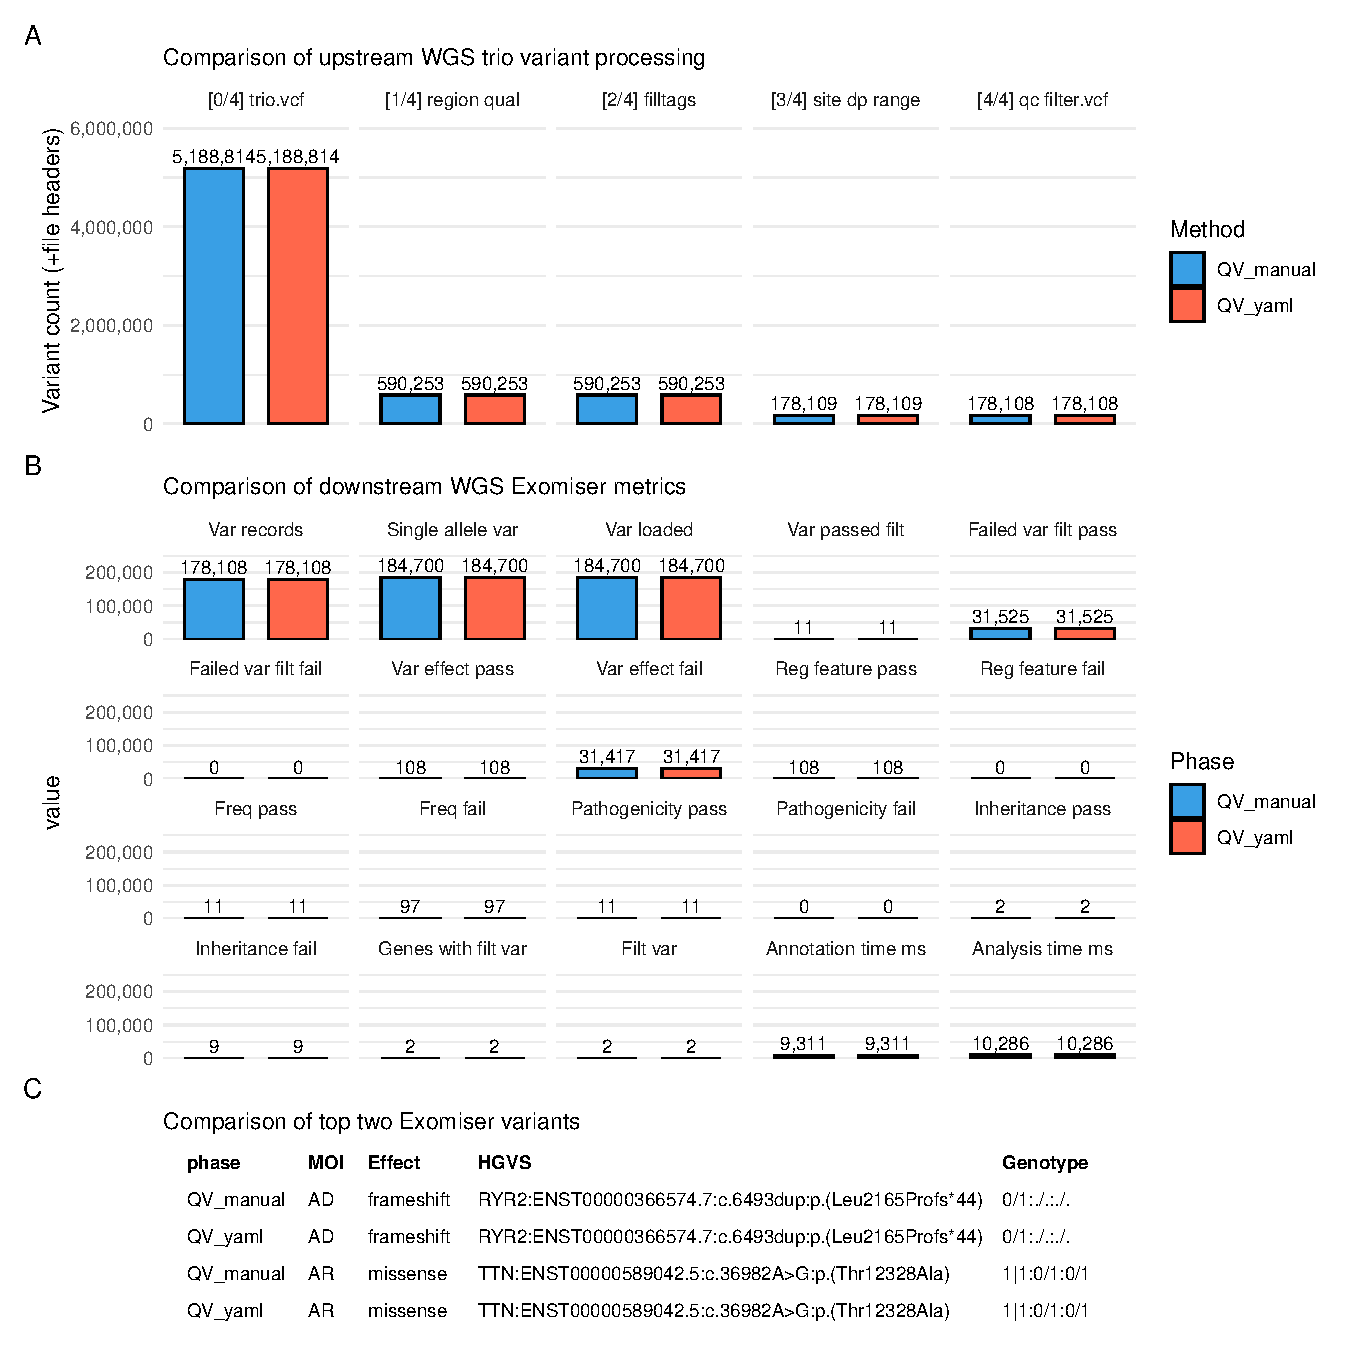
\includegraphics[width=\textwidth]{./images/qv_exomiser/exomiser_validation_bars_facet_metric.pdf}
\caption{\DIFaddFL{Validation of the trio Exomiser pipeline using }\ac{qv} \DIFaddFL{parameterisation. 
}\textbf{\DIFaddFL{(A)}} \DIFaddFL{summarises upstream processing counts by file, 
}\textbf{\DIFaddFL{(B)}} \DIFaddFL{compares downstream Exomiser metrics, 
and }\textbf{\DIFaddFL{(C)}} \DIFaddFL{shows the key variant fields for the two variants identified. 
Variant counts in all panels confirm that intermediate files and final outputs are identical between configurations. 
The five preprocessing stages shown in~(A) are: 
(0) input trio VCF, (1) gene panel region and quality filtering, (2) tag annotation, (3) site-level depth range filtering, and (4) final QC-filtered VCF. 
MOI, mode of inheritance; HGVS, Human Genome Variation Society nomenclature.}}
\label{fig:qv_exomiser_validation}
\end{figure}

\FloatBarrier
\subsection{\DIFadd{Computational benchmark}}\label{sec:benchmark}
\DIFadd{Runtime performance was equivalent between traditional and }\ac{qv}\DIFadd{-based pipelines, as both read identical parameters from different sources. In the WGS trio validation study, pre-processing steps including filtering, }\ac{qc}\DIFadd{, and gene panel selection completed in 16–17~seconds, with a median difference of \textasciitilde0.5~seconds favouring the }\ac{qv} \DIFadd{YAML pipeline (}\textbf{\DIFadd{Figure \ref{fig:benchmark_preprocess_time_bars_by_step_elapsed}}}\DIFadd{). An incidental one-off 5~second delay arose from Singularity initialisation for the }\texttt{\DIFadd{yq}} \DIFadd{utility (step~0), a system-specific effect on our HPC and unrelated to the framework itself.
}

\begin{figure}[h]
\centering
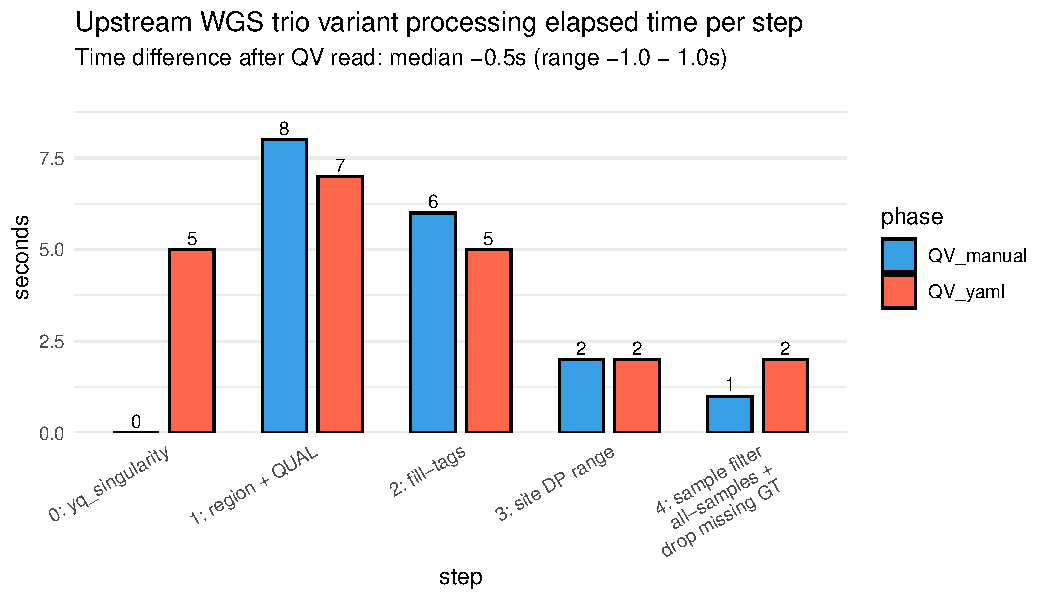
\includegraphics[width=\textwidth]{./images/qv_exomiser/benchmark_preprocess_time_bars_by_step_elapsed.pdf}
\caption{\DIFaddFL{Benchmark of upstream preprocessing times in the WGS trio pipeline comparing }\ac{qv}\DIFaddFL{-based and traditional (manually parameterised) configurations. Stepwise elapsed times were nearly identical across both methods (median difference \textasciitilde0.5~s), with a fixed 5~s overhead from optional Singularity initialisation of }\texttt{\DIFaddFL{yq}} \DIFaddFL{in the }\ac{qv} \DIFaddFL{pipeline. The four preprocessing steps correspond to: (1) gene panel region and quality filtering of the trio VCF, (2) annotation of variant tags, (3) site-level depth range filtering, and (4) per-sample genotype filtering and exclusion of missing genotypes. All steps used }\texttt{\DIFaddFL{BCFtools}} \DIFaddFL{on VCF preprocessing, as illustrated in }\textbf{\DIFaddFL{Figure~\ref{fig:qv_exomiser_validation} (A)}}\DIFaddFL{.}}
\label{fig:benchmark_preprocess_time_bars_by_step_elapsed}
\end{figure}



\subsection{\DIFadd{How to build a QV file}}

\DIFadd{We recommend YAML or JSON for portability and adoption. You can build a QV in three ways:
}

\subsubsection*{\DIFadd{Option 1: use the HTML QV builder (Zenodo)}}
\begin{enumerate}
\item \DIFadd{Open the HTML builder from the Zenodo repository.
}\item \DIFadd{Enter simple }\texttt{\DIFadd{key=value}} \DIFadd{statements in the left pane.
}\item \DIFadd{Copy or download the generated YAML.
}\end{enumerate}

\noindent \DIFadd{Example input lines:
}\DIFmodbegin
\begin{DIFverbatim}[alsolanguage=DIFcode]
%DIF > meta qv_set_id="qv_gwas_common_v1_20250827"
%DIF > meta version="1.0.0"
%DIF > meta title="GWAS common QC"
%DIF > meta authors=Alice,Bob
%DIF > meta tags=GWAS,QC,PCA
%DIF > filter maf_minimum field=MAF operator=">=" value=0.01 desc="Minimum MAF"
%DIF > filter hwe field=HWE_P operator=">=" value=1e-6 logic=keep_if
%DIF > filter region_include desc="include panel" field=OVERLAP(targets.exome.bed) 
%DIF >     >>>> operator=">=" value=1 logic=keep_if
%DIF > criteria disease_panel logic=and desc="HIGH impact within panel"
%DIF > criteria disease_panel field=IMPACT operator="==" value=HIGH
%DIF > criteria disease_panel field=OVERLAP(targets.exome.bed) operator=">=" value=1
%DIF > meta description_patient=
%DIF >     >>>> "There is a strong family history of early heart attacks."
%DIF > meta description_ppie=
%DIF >     >>>> "The PPIE group reviewed and approved the criteria on 2025-08-15."
\end{DIFverbatim}
\DIFmodend

\subsubsection*{\DIFadd{Option 2: write YAML by hand}}
\DIFadd{Minimal pattern:
}\DIFmodbegin
\begin{DIFverbatim}[alsolanguage=DIFcode]
%DIF > meta:
%DIF >   qv_set_id: qv_disease_panel_v1_20250828
%DIF >   version: 1.0.0
%DIF >   title: Disease panel filter
%DIF > filters:
%DIF >   region_include:
%DIF >     description: Restrict to curated disease gene panel
%DIF >     logic: keep_if
%DIF >     field: OVERLAP(targets.disease_panel.bed)
%DIF >     operator: ">="
%DIF >     value: 1
%DIF > criteria:
%DIF >   pathogenic:
%DIF >     description: Variant classified as pathogenic or likely pathogenic
%DIF >     logic: and
%DIF >     conditions:
%DIF >       - group: any_of:start
%DIF >       - { field: CLASS, operator: "==", value: P }
%DIF >       - { field: CLASS, operator: "==", value: LP }
%DIF >       - group: any_of:end
%DIF > notes:
%DIF >   - Gene panel file defines the target regions
\end{DIFverbatim}
\DIFmodend

\subsubsection*{\DIFadd{Option 3: write JSON}}
\DIFadd{JSON equivalent of the minimal example:
}\DIFmodbegin
\begin{DIFverbatim}[alsolanguage=DIFcode]
%DIF > {
%DIF >   "meta": {
%DIF >     "qv_set_id": "qv_disease_panel_v1_20250828",
%DIF >     "version": "1.0.0",
%DIF >     "title": "Disease panel filter"
%DIF >   },
%DIF >   "filters": {
%DIF >     "region_include": {
%DIF >       "description": "Restrict to curated disease gene panel",
%DIF >       "logic": "keep_if",
%DIF >       "field": "OVERLAP(targets.disease_panel.bed)",
%DIF >       "operator": ">=",
%DIF >       "value": 1
%DIF >     }
%DIF >   },
%DIF >   "criteria": {
%DIF >     "pathogenic": {
%DIF >       "description": "Variant classified as pathogenic or likely pathogenic",
%DIF >       "logic": "and",
%DIF >       "conditions": [
%DIF >         { "group": "any_of:start" },
%DIF >         { "field": "CLASS", "operator": "==", "value": "P" },
%DIF >         { "field": "CLASS", "operator": "==", "value": "LP" },
%DIF >         { "group": "any_of:end" }
%DIF >       ]
%DIF >     }
%DIF >   },
%DIF >   "notes": [
%DIF >     "Gene panel file defines the target regions"
%DIF >   ]
%DIF > }
\end{DIFverbatim}
\DIFmodend

\subsubsection*{\DIFadd{Checksum and register}}

\DIFadd{Record the checksum and  register the release:
}

\DIFmodbegin
\begin{DIFverbatim}[alsolanguage=DIFcode]
%DIF > sha256sum qv/examples/qv_disease_panel_v1_20250828.yaml
\end{DIFverbatim}
\DIFmodend

\DIFmodbegin
\begin{DIFverbatim}[alsolanguage=DIFcode]
%DIF > # qv/registry/releases.csv
%DIF > qv_set_id, version, checksum, file, date
%DIF > qv_disease_panel_v1_20250828,1.0.0, ef6cf810b994..., 
%DIF >     > qv_disease_panel_v1_20250828.yaml, 2025-08-28
\end{DIFverbatim}
\DIFmodend

\subsubsection*{\DIFadd{Versioning and IDs}}
\DIFadd{Use a stable }\texttt{\DIFadd{qv\_set\_id}} \DIFadd{plus semantic version.  
Update the version on any change that affects selection or interpretation.  
Keep one file per release and never mutate published files.
}

\subsubsection*{\DIFadd{Use in a workflow}}
\DIFadd{Point your pipeline to the QV file:
}\DIFmodbegin
\begin{DIFverbatim}[alsolanguage=DIFcode]
%DIF > # workflows/.../config.yaml
%DIF > qv_file: ".../qv/registry/qv_disease_panel_v1_20250828.yaml"
\end{DIFverbatim}
\DIFmodend

\DIFadd{It can be read programmatically at runtime, for example using }\texttt{\DIFadd{yq}} \DIFadd{in shell-based workflows or }\texttt{\DIFadd{yaml::read\_yaml()}} \DIFadd{in R, providing the same parameters that would otherwise be embedded within pipeline configurations.
}\DIFaddend 

\end{document}
